\documentclass[12pt]{article}
\usepackage{lmodern}
\usepackage{amssymb,amsmath}
\usepackage{ifxetex,ifluatex}
\usepackage{fixltx2e} % provides \textsubscript
\ifnum 0\ifxetex 1\fi\ifluatex 1\fi=0 % if pdftex
  \usepackage[T1]{fontenc}
  \usepackage[utf8]{inputenc}
\else % if luatex or xelatex
  \ifxetex
    \usepackage{mathspec}
  \else
    \usepackage{fontspec}
  \fi
  \defaultfontfeatures{Ligatures=TeX,Scale=MatchLowercase}
    \setmainfont[]{Arial}
\fi
% use upquote if available, for straight quotes in verbatim environments
\IfFileExists{upquote.sty}{\usepackage{upquote}}{}
% use microtype if available
\IfFileExists{microtype.sty}{%
\usepackage[]{microtype}
\UseMicrotypeSet[protrusion]{basicmath} % disable protrusion for tt fonts
}{}
\PassOptionsToPackage{hyphens}{url} % url is loaded by hyperref
\usepackage[unicode=true]{hyperref}
\hypersetup{
            pdftitle={Guide to the Cumulative CCES Policy Preferences},
            pdfauthor={Angelo Dagonel},
            pdfborder={0 0 0},
            breaklinks=true}
\urlstyle{same}  % don't use monospace font for urls
\usepackage[margin=3cm]{geometry}
\usepackage{graphicx,grffile}
\makeatletter
\def\maxwidth{\ifdim\Gin@nat@width>\linewidth\linewidth\else\Gin@nat@width\fi}
\def\maxheight{\ifdim\Gin@nat@height>\textheight\textheight\else\Gin@nat@height\fi}
\makeatother
% Scale images if necessary, so that they will not overflow the page
% margins by default, and it is still possible to overwrite the defaults
% using explicit options in \includegraphics[width, height, ...]{}
\setkeys{Gin}{width=\maxwidth,height=\maxheight,keepaspectratio}
\IfFileExists{parskip.sty}{%
\usepackage{parskip}
}{% else
\setlength{\parindent}{0pt}
\setlength{\parskip}{6pt plus 2pt minus 1pt}
}
\setlength{\emergencystretch}{3em}  % prevent overfull lines
\providecommand{\tightlist}{%
  \setlength{\itemsep}{0pt}\setlength{\parskip}{0pt}}
\setcounter{secnumdepth}{5}
% Redefines (sub)paragraphs to behave more like sections
\ifx\paragraph\undefined\else
\let\oldparagraph\paragraph
\renewcommand{\paragraph}[1]{\oldparagraph{#1}\mbox{}}
\fi
\ifx\subparagraph\undefined\else
\let\oldsubparagraph\subparagraph
\renewcommand{\subparagraph}[1]{\oldsubparagraph{#1}\mbox{}}
\fi

% set default figure placement to htbp
\makeatletter
\def\fps@figure{htbp}
\makeatother

\usepackage{dcolumn}\usepackage{setspace}\singlespacing\usepackage{graphicx}\usepackage{caption}\captionsetup[table]{skip=10pt}\hypersetup{colorlinks=true,urlcolor=blue,linkcolor=black}
\usepackage{booktabs}
\usepackage{longtable}
\usepackage{array}
\usepackage{multirow}
\usepackage[table]{xcolor}
\usepackage{wrapfig}
\usepackage{float}
\usepackage{colortbl}
\usepackage{pdflscape}
\usepackage{tabu}
\usepackage{threeparttable}
\usepackage{threeparttablex}
\usepackage[normalem]{ulem}
\usepackage{makecell}

\title{Guide to the Cumulative CCES Policy Preferences}
\author{Angelo Dagonel\footnote{PhD student, Department of Government, Harvard
  University. Thanks to Shiro Kuriwaki, Stephen Ansolabehere and Brian
  Schaffner for their suggestions and guidance. Bug reports are welcome
  at the data set's
  \href{https://github.com/psjello/cumulative_cces_policy_preferences}{GitHub
  repository}.}}
\date{Guide last updated: 2021-01-22}

\begin{document}
\maketitle

\begin{quote}
Dagonel, Angelo, 2021, ``Cumulative CCES Policy Preferences'',
\href{https://dataverse.harvard.edu/dataset.xhtml?persistentId=doi:10.7910/DVN/OSXDQO}{\url{doi:10.7910/DVN/OSXDQO}},
Harvard Dataverse.
\end{quote}

Each year, the Cooperative Congressional Election Study (CCES) asks
respondents about their preferences on issues like abortion,
immigration, the environment and more. However, variable names for
question items often change from year to year.

\medskip
The \textbf{Cumulative CCES Policy Preferences} data set compiles
various policy preference question items from CCES respondents over
time. This represents an effort to track, rename, recode, and append
together responses to 43 policy preference question items from
individual CCES survey data sets ranging from 2006 to 2019. The
resulting time series is
\href{https://dataverse.harvard.edu/dataset.xhtml?persistentId=doi:10.7910/DVN/OSXDQO}{available
in an 89 MB data set}. This data set can be combined with demographic
and political information of each respondent from the
\href{https://dataverse.harvard.edu/dataset.xhtml?persistentId=doi:10.7910/DVN/II2DB6}{Cumulative
CCES Common Content} by merging on the \texttt{case\_id} and
\texttt{year} variables.

\medskip
This guide provides details on each policy preference question item,
including the years where an item appears, frequency tables for response
values, and it's unique, year-specific variable name and question
wording.

\section{Usage warnings}\label{usage-warnings}

R users are advised to download and use the .dta version of the data
set, as the .tab version replaces informative value labels with numbers.
To use .dta files in R, install and load the package ``haven'' via the
following lines of code:
\texttt{install.packages("haven");\ library(haven)}.

\medskip
Some question wording varies slightly across time, with more extreme
changes warranting a note at the end of each question item's section.
Further, some item response values are shortened and/or slightly
re-worded from their original values out of convenience. When shortening
and re-wording occurs, the original value wording is listed inside the
item's respective question wording table.

\medskip
Users of the Cumulative CCES Policy Preferences dataset are encouraged
to reference this guide to examine details on any interested question
item before use.

\newpage

\tableofcontents

\section{Question item availability by survey
year}\label{question-item-availability-by-survey-year}

\begin{table}[H]
\centering\rowcolors{2}{gray!6}{white}

\resizebox{\linewidth}{!}{
\begin{tabular}{lcccccccccccccl}
\hiderowcolors
\toprule
Common variable name & 2006 & 2007 & 2008 & 2009 & 2010 & 2011 & 2012 & 2013 & 2014 & 2015 & 2016 & 2017 & 2018 & 2019\\
\midrule
\showrowcolors
abortion\_scale & $\checkmark$ & $\checkmark$ & $\checkmark$ & $\checkmark$ & $\checkmark$ & $\checkmark$ & $\checkmark$ & $\checkmark$ &  &  &  &  &  & \\
abortion\_always &  &  &  &  &  &  &  &  & $\checkmark$ & $\checkmark$ & $\checkmark$ & $\checkmark$ & $\checkmark$ & $\checkmark$\\
abortion\_conditional &  &  &  &  &  &  &  &  & $\checkmark$ & $\checkmark$ & $\checkmark$ & $\checkmark$ & $\checkmark$ & $\checkmark$\\
abortion\_20weeks &  &  &  &  &  &  &  &  & $\checkmark$ & $\checkmark$ & $\checkmark$ & $\checkmark$ & $\checkmark$ & $\checkmark$\\
abortion\_coverage &  &  &  &  &  &  &  &  & $\checkmark$ & $\checkmark$ & $\checkmark$ & $\checkmark$ & $\checkmark$ & \\
abortion\_expenditures &  &  &  &  &  &  &  &  & $\checkmark$ & $\checkmark$ & $\checkmark$ & $\checkmark$ & $\checkmark$ & $\checkmark$\\
abortion\_prohibition &  &  &  &  &  &  &  &  &  & $\checkmark$ & $\checkmark$ & $\checkmark$ & $\checkmark$ & $\checkmark$\\
enviro\_scale & $\checkmark$ & $\checkmark$ &  & $\checkmark$ & $\checkmark$ & $\checkmark$ & $\checkmark$ &  &  &  &  &  &  & \\
enviro\_vs\_jobs & $\checkmark$ & $\checkmark$ & $\checkmark$ &  & $\checkmark$ &  & $\checkmark$ & $\checkmark$ &  &  &  &  &  & \\
enviro\_35mpg &  &  &  &  &  &  &  &  & $\checkmark$ & $\checkmark$ & $\checkmark$ & $\checkmark$ & $\checkmark$ & \\
enviro\_airwateracts &  &  &  &  &  &  &  &  & $\checkmark$ & $\checkmark$ & $\checkmark$ & $\checkmark$ & $\checkmark$ & $\checkmark$\\
enviro\_carbon &  &  &  &  &  &  &  &  & $\checkmark$ & $\checkmark$ & $\checkmark$ & $\checkmark$ & $\checkmark$ & $\checkmark$\\
enviro\_renewable &  &  &  &  &  &  &  &  & $\checkmark$ & $\checkmark$ & $\checkmark$ & $\checkmark$ & $\checkmark$ & $\checkmark$\\
guns\_scale &  &  &  &  & $\checkmark$ &  & $\checkmark$ &  &  &  &  &  &  & \\
guns\_assaultban &  &  &  &  &  &  &  & $\checkmark$ & $\checkmark$ & $\checkmark$ & $\checkmark$ & $\checkmark$ & $\checkmark$ & $\checkmark$\\
guns\_bgchecks &  &  &  &  &  &  &  & $\checkmark$ & $\checkmark$ & $\checkmark$ & $\checkmark$ & $\checkmark$ & $\checkmark$ & $\checkmark$\\
guns\_names &  &  &  &  &  &  &  & $\checkmark$ & $\checkmark$ & $\checkmark$ & $\checkmark$ & $\checkmark$ &  & \\
guns\_permits &  &  &  &  &  &  &  & $\checkmark$ & $\checkmark$ & $\checkmark$ & $\checkmark$ & $\checkmark$ & $\checkmark$ & $\checkmark$\\
immig\_legalize &  & $\checkmark$ &  &  & $\checkmark$ & $\checkmark$ & $\checkmark$ & $\checkmark$ & $\checkmark$ & $\checkmark$ & $\checkmark$ & $\checkmark$ &  & $\checkmark$\\
immig\_border &  & $\checkmark$ &  &  & $\checkmark$ & $\checkmark$ & $\checkmark$ & $\checkmark$ & $\checkmark$ & $\checkmark$ & $\checkmark$ & $\checkmark$ & $\checkmark$ & $\checkmark$\\
immig\_police &  &  &  &  & $\checkmark$ & $\checkmark$ & $\checkmark$ & $\checkmark$ & $\checkmark$ & $\checkmark$ &  & $\checkmark$ &  & \\
immig\_employer &  & $\checkmark$ &  &  & $\checkmark$ &  & $\checkmark$ & $\checkmark$ & $\checkmark$ & $\checkmark$ & $\checkmark$ & $\checkmark$ &  & \\
immig\_services &  &  &  &  &  &  & $\checkmark$ & $\checkmark$ & $\checkmark$ &  &  &  &  & \\
military\_democracy & $\checkmark$ & $\checkmark$ & $\checkmark$ &  & $\checkmark$ & $\checkmark$ & $\checkmark$ & $\checkmark$ & $\checkmark$ & $\checkmark$ & $\checkmark$ &  &  & \\
military\_genocide & $\checkmark$ & $\checkmark$ & $\checkmark$ &  & $\checkmark$ & $\checkmark$ & $\checkmark$ & $\checkmark$ & $\checkmark$ & $\checkmark$ & $\checkmark$ &  &  & \\
military\_helpun & $\checkmark$ & $\checkmark$ & $\checkmark$ &  & $\checkmark$ & $\checkmark$ & $\checkmark$ & $\checkmark$ & $\checkmark$ & $\checkmark$ & $\checkmark$ &  &  & \\
military\_oil & $\checkmark$ & $\checkmark$ & $\checkmark$ &  & $\checkmark$ & $\checkmark$ & $\checkmark$ & $\checkmark$ & $\checkmark$ & $\checkmark$ & $\checkmark$ &  &  & \\
military\_protectallies & $\checkmark$ & $\checkmark$ & $\checkmark$ &  & $\checkmark$ & $\checkmark$ & $\checkmark$ & $\checkmark$ & $\checkmark$ & $\checkmark$ & $\checkmark$ &  &  & \\
military\_terroristcamp & $\checkmark$ & $\checkmark$ & $\checkmark$ &  & $\checkmark$ & $\checkmark$ & $\checkmark$ & $\checkmark$ & $\checkmark$ & $\checkmark$ & $\checkmark$ &  &  & \\
spending\_vs\_tax & $\checkmark$ & $\checkmark$ & $\checkmark$ &  & $\checkmark$ & $\checkmark$ & $\checkmark$ & $\checkmark$ & $\checkmark$ & $\checkmark$ & $\checkmark$ & $\checkmark$ &  & \\
spending\_cuts\_most & $\checkmark$ & $\checkmark$ & $\checkmark$ &  & $\checkmark$ & $\checkmark$ & $\checkmark$ & $\checkmark$ & $\checkmark$ & $\checkmark$ &  & $\checkmark$ &  & \\
spending\_cuts\_least & $\checkmark$ & $\checkmark$ & $\checkmark$ &  & $\checkmark$ & $\checkmark$ & $\checkmark$ & $\checkmark$ & $\checkmark$ & $\checkmark$ &  & $\checkmark$ &  & \\
spending\_welfare &  &  &  &  &  &  &  &  &  &  & $\checkmark$ &  & $\checkmark$ & \\
spending\_healthcare &  &  &  &  &  &  &  &  &  &  & $\checkmark$ &  & $\checkmark$ & \\
spending\_education &  &  &  &  &  &  &  &  &  &  & $\checkmark$ &  & $\checkmark$ & \\
spending\_police &  &  &  &  &  &  &  &  &  &  & $\checkmark$ &  & $\checkmark$ & \\
spending\_infrastructure &  &  &  &  &  &  &  &  &  &  & $\checkmark$ &  & $\checkmark$ & \\
affirmativeaction\_scale & $\checkmark$ & $\checkmark$ &  &  &  &  &  &  &  &  &  &  &  & \\
affirmativeaction &  &  & $\checkmark$ & $\checkmark$ & $\checkmark$ & $\checkmark$ & $\checkmark$ & $\checkmark$ & $\checkmark$ &  &  &  &  & \\
gaymarriage\_scale & $\checkmark$ & $\checkmark$ &  &  &  &  &  &  &  &  &  &  &  & \\
gaymarriage &  &  & $\checkmark$ & $\checkmark$ & $\checkmark$ & $\checkmark$ & $\checkmark$ & $\checkmark$ & $\checkmark$ & $\checkmark$ & $\checkmark$ &  &  & \\
incometax\_vs\_salestax & $\checkmark$ & $\checkmark$ & $\checkmark$ &  & $\checkmark$ & $\checkmark$ & $\checkmark$ & $\checkmark$ & $\checkmark$ & $\checkmark$ & $\checkmark$ & $\checkmark$ &  & \\
repealaca &  &  &  &  &  &  & $\checkmark$ & $\checkmark$ & $\checkmark$ & $\checkmark$ & $\checkmark$ & $\checkmark$ & $\checkmark$ & $\checkmark$\\
\bottomrule
\end{tabular}}
\rowcolors{2}{white}{white}
\end{table}

\newpage

\section{Question items}\label{question-items}

\subsection{Abortion}\label{abortion}

\subsubsection{abortion\_scale}\label{abortion_scale}

Support scale for access to abortion (1 = Never permit, 4 = Always
allow)

Years in data: 2006, 2007, 2008, 2009, 2010, 2011, 2012,
2013\begingroup\fontsize{10}{12}\selectfont

\begin{longtable}[t]{lcccccccc}
\caption{\label{tab:unnamed-chunk-4}abortion\_scale: Frequency table}\\
\toprule
Response & 2006 & 2007 & 2008 & 2009 & 2010 & 2011 & 2012 & 2013\\
\midrule
\endfirsthead
\caption[]{abortion\_scale: Frequency table \textit{(continued)}}\\
\toprule
Response & 2006 & 2007 & 2008 & 2009 & 2010 & 2011 & 2012 & 2013\\
\midrule
\endhead
\
\endfoot
\bottomrule
\endlastfoot
Never permit & 3,481 & 862 & 3,774 & 1,793 & 6,623 & 2,448 & 5,684 & 1,873\\
Permit in rape, incest cases & 9,120 & 2,260 & 7,485 & 4,402 & 15,641 & 5,399 & 14,146 & 4,169\\
Permit in other cases & 5,466 & 1,461 & 3,661 & 1,866 & 8,135 & 2,888 & 7,174 & 2,272\\
Always allow & 15,877 & 4,677 & 10,698 & 5,657 & 24,639 & 9,415 & 27,111 & 7,963\\*
\end{longtable}

\endgroup{}

Year-specific variable names and wording

\begin{longtable}[t]{rl>{\raggedright\arraybackslash}p{10cm}}
\caption{\label{tab:unnamed-chunk-4}abortion\_scale: Year-specific wording}\\
\toprule
Year & Variable & Question wording\\
\midrule
\endfirsthead
\caption[]{abortion\_scale: Year-specific wording \textit{(continued)}}\\
\toprule
Year & Variable & Question wording\\
\midrule
\endhead
\
\endfoot
\bottomrule
\endlastfoot
2006 & v3019 & There has been some discussion about abortion during recent years.  Which one of the opinions on this page best agrees with your view on this issue? [1 By law, abortion should never be permitted, 2 The law should permit abortion only in case of rape, incest or when the woman's life is in danger, 3 The law should permit abortion for reasons other than rape, incest, or danger to the woman's  life, but only after the need for the abortion has been clearly established, 4 By law, a woman should always be able to  obtain an abortion as a matter of personal choice]\\
2007 & CC06\_V3019 & There has been some discussion about abortion during recent years. Which one of the opinions on this page best agrees with your view on this issue? [1 By law, abortion should never be permitted, 2 The law should permit abortion only in case of rape, incest, 3 The law should permit abortion for reasons other than rape, 4 By law, a woman should always be able to obtain an abortion]\\
2008 & cc310 & Which one of the opinions on this page best agrees with your view on abortion? [1 By law, abortion should never be permitted, 2 The law should permit abortion only in case of rape, incest or when the womans life is in danger, 3 The law should permit abortion for reasons other than rape, incest, or danger to the womans life, but only after the need for the abortion has been clearly established, 4 By law, a woman should always be able to obtain an abortion as a matter of personal choice]\\
2009 & cc09\_53 & Abortion\\
2010 & CC324 & Which one of the opinions on this page best agrees with your view on abortion? [1 By law, abortion should never be permitted, 2 The law should permit abortion only in case of rape, incest or when the womans life is in danger, 3 The law should permit abortion for reasons other than rape, incest, or danger to the womans life, but only after the need for the abortion has been clearly established, 4 By law, a woman should always be able to obtain an abortion as a matter of personal choice]\\
2011 & CC352 & Abortion\\
2012 & CC324 & Which one of the opinions on this page best agrees with your view on abortion? [1 By law, abortion should never be permitted, 2 The law should permit abortion only in case of rape, incest or when the womans life is in danger, 3 The law should permit abortion for reasons other than rape, incest, or danger to the womans life, but only after the need for the abortion has been clearly established, 4 By law, a woman should always be able to obtain an abortion as a matter of personal choice]\\
2013 & CC327 & Which one of the opinions on this page best agrees with your view on abortion? [1 By law, abortion should never bepermitted, 2 The law should permit abortion only incase of rape, incest or when thewoman's life is in danger, 3 The law should permit abortion forreasons other than rape, incest, ordanger to the woman's life, but onlyafter the need for the abortion has beenclearly established, 4 By law, a woman should always be ableto obtain an abortion as a matter ofpersonal choice]\\*
\end{longtable}

\subsubsection{abortion\_always}\label{abortion_always}

Always allow abortion

Years in data: 2014, 2015, 2016, 2017, 2018,
2019\begingroup\fontsize{10}{12}\selectfont

\begin{longtable}[t]{lcccccc}
\caption{\label{tab:unnamed-chunk-4}abortion\_always: Frequency table}\\
\toprule
Response & 2014 & 2015 & 2016 & 2017 & 2018 & 2019\\
\midrule
\endfirsthead
\caption[]{abortion\_always: Frequency table \textit{(continued)}}\\
\toprule
Response & 2014 & 2015 & 2016 & 2017 & 2018 & 2019\\
\midrule
\endhead
\
\endfoot
\bottomrule
\endlastfoot
Support & 33,283 & 7,907 & 39,808 & 10,741 & 35,751 & 10,067\\
Oppose & 22,395 & 6,200 & 24,730 & 7,444 & 24,150 & 7,841\\*
\end{longtable}

\endgroup{}

Year-specific variable names and wording

\begin{longtable}[t]{rl>{\raggedright\arraybackslash}p{10cm}}
\caption{\label{tab:unnamed-chunk-4}abortion\_always: Year-specific wording}\\
\toprule
Year & Variable & Question wording\\
\midrule
\endfirsthead
\caption[]{abortion\_always: Year-specific wording \textit{(continued)}}\\
\toprule
Year & Variable & Question wording\\
\midrule
\endhead
\
\endfoot
\bottomrule
\endlastfoot
2014 & CC14\_323\_1 & Do you support or oppose each of the following proposals? . . . Always allow a woman to obtain an abortion as a matter of choice\\
2015 & CC15\_322a & Do you support or oppose each of the following proposals? Always allow a woman to obtain an abortion as a matter of choice\\
2016 & CC16\_332a & Do you support or oppose each of the following proposals? Always allow a woman to obtain an abortion as a matter of choice\\
2017 & CC17\_332a & Do you support or oppose each of the following proposals? Always allow a woman to obtain an abortion as a matter of choice\\
2018 & CC18\_321a & Do you support or oppose each of the following proposals? Always allow a woman to obtain an abortion as a matter of choice\\
2019 & CC19\_321a & Always allow a woman to obtain an abortion as a matter of choice\\*
\end{longtable}

\subsubsection{abortion\_conditional}\label{abortion_conditional}

Allow abortion only under certain cases

Years in data: 2014, 2015, 2016, 2017, 2018,
2019\begingroup\fontsize{10}{12}\selectfont

\begin{longtable}[t]{lcccccc}
\caption{\label{tab:unnamed-chunk-4}abortion\_conditional: Frequency table}\\
\toprule
Response & 2014 & 2015 & 2016 & 2017 & 2018 & 2019\\
\midrule
\endfirsthead
\caption[]{abortion\_conditional: Frequency table \textit{(continued)}}\\
\toprule
Response & 2014 & 2015 & 2016 & 2017 & 2018 & 2019\\
\midrule
\endhead
\
\endfoot
\bottomrule
\endlastfoot
Support & 26,198 & 6,247 & 29,616 & 7,729 & 24,315 & 7,572\\
Oppose & 29,166 & 7,822 & 34,892 & 10,452 & 35,583 & 10,395\\*
\end{longtable}

\endgroup{}

Year-specific variable names and wording

\begin{longtable}[t]{rl>{\raggedright\arraybackslash}p{10cm}}
\caption{\label{tab:unnamed-chunk-4}abortion\_conditional: Year-specific wording}\\
\toprule
Year & Variable & Question wording\\
\midrule
\endfirsthead
\caption[]{abortion\_conditional: Year-specific wording \textit{(continued)}}\\
\toprule
Year & Variable & Question wording\\
\midrule
\endhead
\
\endfoot
\bottomrule
\endlastfoot
2014 & CC14\_323\_2 & Do you support or oppose each of the following proposals? . . . Permit abortion only in cases of rape, incest, or when the womans life is in danger\\
2015 & CC15\_322b & Do you support or oppose each of the following proposals? Permit abortion ONLY in case of rape, incest or when the woman's life is in danger\\
2016 & CC16\_332b & Do you support or oppose each of the following proposals? Permit abortion only in case of rape, incest or when the woman's life is in danger\\
2017 & CC17\_332b & Do you support or oppose each of the following proposals? Permit abortion only in case of rape, incest or when the woman's life is in danger\\
2018 & CC18\_321b & Do you support or oppose each of the following proposals? Permit abortion ONLY in case of rape, incest or when the woman's life is in danger\\
2019 & CC19\_321b & Permit abortion ONLY in case of rape, incest or when the woman's life is in danger\\*
\end{longtable}

\subsubsection{abortion\_20weeks}\label{abortion_20weeks}

Ban abortion after 20 weeks

Years in data: 2014, 2015, 2016, 2017, 2018,
2019\begingroup\fontsize{10}{12}\selectfont

\begin{longtable}[t]{lcccccc}
\caption{\label{tab:unnamed-chunk-4}abortion\_20weeks: Frequency table}\\
\toprule
Response & 2014 & 2015 & 2016 & 2017 & 2018 & 2019\\
\midrule
\endfirsthead
\caption[]{abortion\_20weeks: Frequency table \textit{(continued)}}\\
\toprule
Response & 2014 & 2015 & 2016 & 2017 & 2018 & 2019\\
\midrule
\endhead
\
\endfoot
\bottomrule
\endlastfoot
Support & 37,103 & 9,676 & 39,057 & 11,675 & 38,280 & 10,910\\
Oppose & 18,318 & 4,391 & 25,461 & 6,506 & 21,634 & 7,079\\*
\end{longtable}

\endgroup{}

Year-specific variable names and wording

\begin{longtable}[t]{rl>{\raggedright\arraybackslash}p{10cm}}
\caption{\label{tab:unnamed-chunk-4}abortion\_20weeks: Year-specific wording}\\
\toprule
Year & Variable & Question wording\\
\midrule
\endfirsthead
\caption[]{abortion\_20weeks: Year-specific wording \textit{(continued)}}\\
\toprule
Year & Variable & Question wording\\
\midrule
\endhead
\
\endfoot
\bottomrule
\endlastfoot
2014 & CC14\_323\_3 & Do you support or oppose each of the following proposals? . . . Prohibit abortions after the 20th week of pregnancy\\
2015 & CC15\_322c & Do you support or oppose each of the following proposals? Ban abortions after the 20th week of pregnancy\\
2016 & CC16\_332c & Do you support or oppose each of the following proposals? Prohibit all abortions after the 20th week of pregnancy\\
2017 & CC17\_332c & Do you support or oppose each of the following proposals? Ban abortions after the 20th week of pregnancy\\
2018 & CC18\_321c & Do you support or oppose each of the following proposals? Ban abortions after the 20th week of pregnancy\\
2019 & CC19\_321c & Ban abortions after the 20th week of pregnancy\\*
\end{longtable}

\subsubsection{abortion\_coverage}\label{abortion_coverage}

Employer coverage of abortion

Years in data: 2014, 2015, 2016, 2017,
2018\begingroup\fontsize{10}{12}\selectfont

\begin{longtable}[t]{lccccc}
\caption{\label{tab:unnamed-chunk-4}abortion\_coverage: Frequency table}\\
\toprule
Response & 2014 & 2015 & 2016 & 2017 & 2018\\
\midrule
\endfirsthead
\caption[]{abortion\_coverage: Frequency table \textit{(continued)}}\\
\toprule
Response & 2014 & 2015 & 2016 & 2017 & 2018\\
\midrule
\endhead
\
\endfoot
\bottomrule
\endlastfoot
Support & 25,366 & 6,856 & 28,138 & 8,225 & 25,999\\
Oppose & 30,273 & 7,246 & 36,400 & 9,960 & 33,938\\*
\end{longtable}

\endgroup{}

Year-specific variable names and wording

\begin{longtable}[t]{rl>{\raggedright\arraybackslash}p{10cm}}
\caption{\label{tab:unnamed-chunk-4}abortion\_coverage: Year-specific wording}\\
\toprule
Year & Variable & Question wording\\
\midrule
\endfirsthead
\caption[]{abortion\_coverage: Year-specific wording \textit{(continued)}}\\
\toprule
Year & Variable & Question wording\\
\midrule
\endhead
\
\endfoot
\bottomrule
\endlastfoot
2014 & CC14\_323\_4 & Do you support or oppose each of the following proposals? . . . Allow employers to decline coverage of abortions in insurance plans\\
2015 & CC15\_322d & Do you support or oppose each of the following proposals? Allow employers to decline coverage of abortions in insurance plans\\
2016 & CC16\_332d & Do you support or oppose each of the following proposals? Allow employers to decline coverage of abortions in insurance plans\\
2017 & CC17\_332d & Do you support or oppose each of the following proposals? Allow employers to decline coverage of abortions in insurance plans\\
2018 & CC18\_321d & Do you support or oppose each of the following proposals? Allow employers to decline coverage of abortions in insurance plans\\*
\end{longtable}

\subsubsection{abortion\_expenditures}\label{abortion_expenditures}

Prohibit expenditures for abortion

Years in data: 2014, 2015, 2016, 2017, 2018,
2019\begingroup\fontsize{10}{12}\selectfont

\begin{longtable}[t]{lcccccc}
\caption{\label{tab:unnamed-chunk-4}abortion\_expenditures: Frequency table}\\
\toprule
Response & 2014 & 2015 & 2016 & 2017 & 2018 & 2019\\
\midrule
\endfirsthead
\caption[]{abortion\_expenditures: Frequency table \textit{(continued)}}\\
\toprule
Response & 2014 & 2015 & 2016 & 2017 & 2018 & 2019\\
\midrule
\endhead
\
\endfoot
\bottomrule
\endlastfoot
Support & 26,497 & 7,032 & 29,217 & 8,253 & 26,280 & 9,127\\
Oppose & 28,968 & 7,027 & 35,321 & 9,929 & 33,651 & 8,863\\*
\end{longtable}

\endgroup{}

Year-specific variable names and wording

\begin{longtable}[t]{rl>{\raggedright\arraybackslash}p{10cm}}
\caption{\label{tab:unnamed-chunk-4}abortion\_expenditures: Year-specific wording}\\
\toprule
Year & Variable & Question wording\\
\midrule
\endfirsthead
\caption[]{abortion\_expenditures: Year-specific wording \textit{(continued)}}\\
\toprule
Year & Variable & Question wording\\
\midrule
\endhead
\
\endfoot
\bottomrule
\endlastfoot
2014 & CC14\_323\_5 & Do you support or oppose each of the following proposals? . . . Prohibit the expenditure of funds authorized or appropriated by federal law for any abortion\\
2015 & CC15\_322e & Do you support or oppose each of the following proposals? Prohibit the expenditure of funds authorized or appropriated by federal law for any abortion.\\
2016 & CC16\_332e & Do you support or oppose each of the following proposals? Prohibit the expenditure of funds authorized or appropriated by federal law for any abortion\\
2017 & CC17\_332e & Do you support or oppose each of the following proposals? Prohibit the expenditure of funds authorized or appropriated by federal law for any abortion.\\
2018 & CC18\_321e & Do you support or oppose each of the following proposals? Prohibit the expenditure of funds authorized or appropriated by federal law for any abortion.\\
2019 & CC19\_321d & Prohibit the expenditure of funds authorized or appropriated by federal law for any abortion except to save the life of the woman, or if the pregnancy arises from incest or rape\\*
\end{longtable}

\subsubsection{abortion\_prohibition}\label{abortion_prohibition}

Total prohibition of abortion

Years in data: 2015, 2016, 2017, 2018,
2019\begingroup\fontsize{10}{12}\selectfont

\begin{longtable}[t]{lccccc}
\caption{\label{tab:unnamed-chunk-4}abortion\_prohibition: Frequency table}\\
\toprule
Response & 2015 & 2016 & 2017 & 2018 & 2019\\
\midrule
\endfirsthead
\caption[]{abortion\_prohibition: Frequency table \textit{(continued)}}\\
\toprule
Response & 2015 & 2016 & 2017 & 2018 & 2019\\
\midrule
\endhead
\
\endfoot
\bottomrule
\endlastfoot
Support & 2,597 & 10,144 & 3,128 & 9,224 & 3,350\\
Oppose & 11,439 & 54,369 & 15,056 & 50,685 & 14,629\\*
\end{longtable}

\endgroup{}

Year-specific variable names and wording

\begin{longtable}[t]{rl>{\raggedright\arraybackslash}p{10cm}}
\caption{\label{tab:unnamed-chunk-4}abortion\_prohibition: Year-specific wording}\\
\toprule
Year & Variable & Question wording\\
\midrule
\endfirsthead
\caption[]{abortion\_prohibition: Year-specific wording \textit{(continued)}}\\
\toprule
Year & Variable & Question wording\\
\midrule
\endhead
\
\endfoot
\bottomrule
\endlastfoot
2015 & CC15\_322f & Do you support or oppose each of the following proposals? Make abortions illegal in all circumstances.\\
2016 & CC16\_332f & Do you support or oppose each of the following proposals? Make abortions illegal in all circumstances\\
2017 & CC17\_332f & Do you support or oppose each of the following proposals? Make abortion illegal in all circumstances.\\
2018 & CC18\_321f & Do you support or oppose each of the following proposals? Make abortion illegal in all circumstances.\\
2019 & CC19\_321e & Make abortions illegal in all circumstances\\*
\end{longtable}\newpage

\subsection{Environment}\label{environment}

\subsubsection{enviro\_scale}\label{enviro_scale}

Opposition scale to climate change (1 = serious problem, 5 = not
occuring)

Years in data: 2006, 2007, 2009, 2010, 2011,
2012\begingroup\fontsize{10}{12}\selectfont

\begin{longtable}[t]{lcccccc}
\caption{\label{tab:unnamed-chunk-4}enviro\_scale: Frequency table}\\
\toprule
Response & 2006 & 2007 & 2009 & 2010 & 2011 & 2012\\
\midrule
\endfirsthead
\caption[]{enviro\_scale: Frequency table \textit{(continued)}}\\
\toprule
Response & 2006 & 2007 & 2009 & 2010 & 2011 & 2012\\
\midrule
\endhead
\
\endfoot
\bottomrule
\endlastfoot
Immediate action & 5,681 & 2,209 & 3,073 & 15,409 & 5,786 & 14,764\\
Some action & 4,287 & 1,486 & 4,205 & 13,853 & 5,778 & 16,378\\
More research needed & 3,646 & 1,307 & 2,743 & 10,730 & 4,085 & 11,461\\
No action necessary & 2,632 & 1,027 & 3,760 & 11,095 & 3,289 & 8,693\\
Climate change not occurring & 0 & 0 & 0 & 4,201 & 1,212 & 3,075\\*
\end{longtable}

\endgroup{}

Year-specific variable names and wording

\begin{longtable}[t]{rl>{\raggedright\arraybackslash}p{10cm}}
\caption{\label{tab:unnamed-chunk-4}enviro\_scale: Year-specific wording}\\
\toprule
Year & Variable & Question wording\\
\midrule
\endfirsthead
\caption[]{enviro\_scale: Year-specific wording \textit{(continued)}}\\
\toprule
Year & Variable & Question wording\\
\midrule
\endhead
\
\endfoot
\bottomrule
\endlastfoot
2006 & v2092 & From what you know about global climate change or global warming, which one of the following statements comes closest to your opinion? [1 Global climate change has been established as a serious problem, and immediate action is necessary. 2 There is enough evidence that climate change is taking place and some action should be taken. 3 We don't know enough about global climate change, and more research is necessary before we take any actions. 4 Concern about global climate change is unwarranted.]\\
2007 & CC06\_V2092 & From what you know about global climate change or global warming, which one of the following statements comes closest to your opinion? [1 Immediate action, 2 Some action, 3 More research, 4 Concern unwarranted]\\
2009 & cc09\_51 & Global Warming\\
2010 & CC321 & From what you know about global climate change or global warming, which one of the following statements comes closest to your opinion? [1 Global climate change has been established as a serious problem, and immediate action is necessary. 2 here is enough evidence that climate change is taking place and some action should be taken. 3 We don’t know enough about global climate change, and more research is necessary before taking any actions. 4 Concern about global climate change is exaggerated. No action is necessary. 5 Global climate change is not occurring; this is not a real issue.]\\
2011 & CC350 & Climate\\
2012 & CC321 & From what you know about global climate change or global warming, which one of the following statements comes closest to your opinion? [1 Global Climate change has been established as a serious problem, and immediate action is necessary. 2 There is enough evidence that climate change is taking place and some action should be taken. 3 We don't know enough about global climate change, and more research is necessary before we take any actions. 4 Concern about global climate chane is exaggerated. No action is necessary. 5 Global climate change is not occurring; this is not a real issue]\\*
\end{longtable}

\emph{Note: From 2010 onward, this question includes a fifth response
option, `Global climate change is not occurring'.}

\subsubsection{enviro\_vs\_jobs}\label{enviro_vs_jobs}

Preference scale between environmental protection and job availability
(1=Environmental protection, 5=Job protection)

Years in data: 2006, 2007, 2008, 2010, 2012,
2013\begingroup\fontsize{10}{12}\selectfont

\begin{longtable}[t]{lcccccc}
\caption{\label{tab:unnamed-chunk-4}enviro\_vs\_jobs: Frequency table}\\
\toprule
Response & 2006 & 2007 & 2008 & 2010 & 2012 & 2013\\
\midrule
\endfirsthead
\caption[]{enviro\_vs\_jobs: Frequency table \textit{(continued)}}\\
\toprule
Response & 2006 & 2007 & 2008 & 2010 & 2012 & 2013\\
\midrule
\endhead
\
\endfoot
\bottomrule
\endlastfoot
Environment much more important & 8,557 & 2,597 & 3,765 & 7,643 & 6,558 & 2,172\\
Environment somewhat more important & 8,908 & 2,442 & 4,917 & 9,802 & 9,602 & 2,874\\
Environment and jobs of same importance & 8,119 & 2,107 & 6,745 & 15,358 & 17,209 & 5,844\\
Jobs somewhat more important & 6,239 & 1,705 & 6,217 & 13,453 & 13,340 & 3,422\\
Jobs much more important & 3,004 & 832 & 4,014 & 8,964 & 7,591 & 2,038\\
Haven't thought much about this & 1,290 & 261 & 0 & 0 & 0 & 0\\*
\end{longtable}

\endgroup{}

Year-specific variable names and wording

\begin{longtable}[t]{rl>{\raggedright\arraybackslash}p{10cm}}
\caption{\label{tab:unnamed-chunk-4}enviro\_vs\_jobs: Year-specific wording}\\
\toprule
Year & Variable & Question wording\\
\midrule
\endfirsthead
\caption[]{enviro\_vs\_jobs: Year-specific wording \textit{(continued)}}\\
\toprule
Year & Variable & Question wording\\
\midrule
\endhead
\
\endfoot
\bottomrule
\endlastfoot
2006 & v3022 & Some people think it is important to protect the environment even if it costs some jobs or otherwise reduces our standard of living. Other people think that protecting the environment is not as important as maintaining jobs and our standard of living.  Which is closer to the way you feel, or haven't you thought much about this?\\
2007 & CC06\_V3022 & Some people think it is important to protect the environment even if it costs some jobs or otherwise reduces our standard of living. Other people think that protecting the environment is not as important as maintaining jobs and our standard of living. Which is closer to the way you feel, or haven't you thought much about this?\\
2008 & cc311 & Some people think it is important to protect the environment even if it costs some jobs or otherwise reduces our standard of living. Other people think that protecting the environment is not as important as maintaining jobs and our standard of living. Which is closer to the way you feel, or haven't you thought much about this?\\
2010 & CC325 & Some people think it is important to protect the environment even if it costs some jobs or otherwise reduces our standard of living. Other people think that protecting the environment is not as important as maintaining jobs and our standard of living. Which is closer to the way you feel, or haven't you thought much about this?\\
2012 & CC325 & Some people think it is important to protect the environment even if it costs some jobs or otherwise reduces our standard of living. Other people think that protecting the environment is not as important as maintaining jobs and our standard of living. Which is closer to the way you feel, or haven’t you thought much about this?\\
2013 & CC328 & Some people think it is important to protect the environment even if it costs some jobs or otherwise reduces our standard of living. Other people think that protecting the environment is not as important as maintaining jobs and our standard of living. Which is closer to the way you feel, or haven't you thought much about this?\\*
\end{longtable}

\emph{Note: In 2006 and 2007, this question includes a sixth response
option, `Haven't thought much about this'.}

\subsubsection{enviro\_35mpg}\label{enviro_35mpg}

Raise fuel efficiency from 25 to 35 mpg

Years in data: 2014, 2015, 2016, 2017,
2018\begingroup\fontsize{10}{12}\selectfont

\begin{longtable}[t]{lccccc}
\caption{\label{tab:unnamed-chunk-4}enviro\_35mpg: Frequency table}\\
\toprule
Response & 2014 & 2015 & 2016 & 2017 & 2018\\
\midrule
\endfirsthead
\caption[]{enviro\_35mpg: Frequency table \textit{(continued)}}\\
\toprule
Response & 2014 & 2015 & 2016 & 2017 & 2018\\
\midrule
\endhead
\
\endfoot
\bottomrule
\endlastfoot
Support & 39,160 & 9,634 & 45,022 & 12,533 & 34,966\\
Oppose & 16,279 & 4,430 & 19,522 & 5,654 & 16,535\\*
\end{longtable}

\endgroup{}

Year-specific variable names and wording

\begin{longtable}[t]{rl>{\raggedright\arraybackslash}p{10cm}}
\caption{\label{tab:unnamed-chunk-4}enviro\_35mpg: Year-specific wording}\\
\toprule
Year & Variable & Question wording\\
\midrule
\endfirsthead
\caption[]{enviro\_35mpg: Year-specific wording \textit{(continued)}}\\
\toprule
Year & Variable & Question wording\\
\midrule
\endhead
\
\endfoot
\bottomrule
\endlastfoot
2014 & CC14\_326\_2 & Raise required fuel efficiency for the average automobile from 25 mpg to 35 mpg.\\
2015 & CC15\_323\_2 & Do you support or oppose each of the following proposals? Raise required fuel efficiency for the average automobile from 25 mpg to 35 mpg.\\
2016 & CC16\_333b & Do you support or oppose each of the following proposals? Raise required fuel efficiency for the average automobile from 25 mpg to 35 mpg.\\
2017 & CC17\_333b & Do you support or oppose each of the following proposals? Raise required fuel efficiency for the average automobile from 25 mpg to 35 mpg.\\
2018 & CC18\_415b & Do you support or oppose each of the following proposals? Lower the required fuel efficiency for the average automobile from 35 mpg to 25 mpg.\\*
\end{longtable}

\emph{Note: In 2018, question wording switches from `Raise required fuel
efficiency\ldots{}from 25 mpg' to `Lower the required fuel
efficiency\ldots{}from 35 mpg'.}

\subsubsection{enviro\_airwateracts}\label{enviro_airwateracts}

Strengthen EPA enforcement of Clean Air and Water acts

Years in data: 2014, 2015, 2016, 2017, 2018,
2019\begingroup\fontsize{10}{12}\selectfont

\begin{longtable}[t]{lcccccc}
\caption{\label{tab:unnamed-chunk-4}enviro\_airwateracts: Frequency table}\\
\toprule
Response & 2014 & 2015 & 2016 & 2017 & 2018 & 2019\\
\midrule
\endfirsthead
\caption[]{enviro\_airwateracts: Frequency table \textit{(continued)}}\\
\toprule
Response & 2014 & 2015 & 2016 & 2017 & 2018 & 2019\\
\midrule
\endhead
\
\endfoot
\bottomrule
\endlastfoot
Support & 27,064 & 7,588 & 37,672 & 11,412 & 30,106 & 11,097\\
Oppose & 28,342 & 6,459 & 26,875 & 6,772 & 21,438 & 6,888\\*
\end{longtable}

\endgroup{}

Year-specific variable names and wording

\begin{longtable}[t]{rl>{\raggedright\arraybackslash}p{10cm}}
\caption{\label{tab:unnamed-chunk-4}enviro\_airwateracts: Year-specific wording}\\
\toprule
Year & Variable & Question wording\\
\midrule
\endfirsthead
\caption[]{enviro\_airwateracts: Year-specific wording \textit{(continued)}}\\
\toprule
Year & Variable & Question wording\\
\midrule
\endhead
\
\endfoot
\bottomrule
\endlastfoot
2014 & CC14\_326\_4 & Environmental Protection Agency strengthening enforcement of the Clean Air Act even if it costs US jobs\\
2015 & CC15\_323\_4 & Do you support or oppose each of the following proposals? Strengthen the Environmental Protection Agency enforcement of the Clean Air Act and Clean Water Act even if costs US jobs\\
2016 & CC16\_333d & Do you support or oppose each of the following proposals? Strengthen enforcement of the Clean Air Act and Clean Water Act even if costs US jobs\\
2017 & CC17\_333d & Do you support or oppose each of the following proposals? Strengthen the Environmental Protection Agency enforcement of the Clean Air Act and Clean Water Act even if it costs U.S. jobs.\\
2018 & CC18\_415d & Do you support or oppose each of the following proposals? Strengthen the Environmental Protection Agency enforcement of the Clean Air Act and Clean Water Act even if it costs US jobs\\
2019 & CC19\_340c & Strengthen the Environmental Protection Agency enforcement of the Clean Air Act and Clean Water Act even if it costs U.S. jobs\\*
\end{longtable}

\subsubsection{enviro\_carbon}\label{enviro_carbon}

Allow EPA to regulate carbon dioxide emissions

Years in data: 2014, 2015, 2016, 2017, 2018,
2019\begingroup\fontsize{10}{12}\selectfont

\begin{longtable}[t]{lcccccc}
\caption{\label{tab:unnamed-chunk-4}enviro\_carbon: Frequency table}\\
\toprule
Response & 2014 & 2015 & 2016 & 2017 & 2018 & 2019\\
\midrule
\endfirsthead
\caption[]{enviro\_carbon: Frequency table \textit{(continued)}}\\
\toprule
Response & 2014 & 2015 & 2016 & 2017 & 2018 & 2019\\
\midrule
\endhead
\
\endfoot
\bottomrule
\endlastfoot
Support & 38,653 & 8,982 & 43,932 & 12,309 & 33,678 & 12,135\\
Oppose & 16,728 & 5,065 & 20,608 & 5,873 & 17,805 & 5,842\\*
\end{longtable}

\endgroup{}

Year-specific variable names and wording

\begin{longtable}[t]{rl>{\raggedright\arraybackslash}p{10cm}}
\caption{\label{tab:unnamed-chunk-4}enviro\_carbon: Year-specific wording}\\
\toprule
Year & Variable & Question wording\\
\midrule
\endfirsthead
\caption[]{enviro\_carbon: Year-specific wording \textit{(continued)}}\\
\toprule
Year & Variable & Question wording\\
\midrule
\endhead
\
\endfoot
\bottomrule
\endlastfoot
2014 & CC14\_326\_1 & Do you support or oppose each of the following policies? Environmental Protection Agency regulating carbon emissions\\
2015 & CC15\_323\_1 & Do you support or oppose each of the following proposals? Give Environmental Protection Agency power to regulate Carbon Dioxide emissions\\
2016 & CC16\_333a & Do you support or oppose each of the following proposals? Give Environmental Protection Agency power to regulate Carbon Dioxide emissions\\
2017 & CC17\_333a & Do you support or oppose each of the following proposals? Give Environmental Protection Agency power to regulate Carbon Dioxide emissions.\\
2018 & CC18\_415a & Do you support or oppose each of the following proposals? Give the Environmental Protection Agency power to regulate Carbon Dioxide emissions\\
2019 & CC19\_340a & Give the Environmental Protection Agency power to regulate Carbon Dioxide emissions\\*
\end{longtable}

\subsubsection{enviro\_renewable}\label{enviro_renewable}

Require states use a minimum amount of renewable fuels

Years in data: 2014, 2015, 2016, 2017, 2018,
2019\begingroup\fontsize{10}{12}\selectfont

\begin{longtable}[t]{lcccccc}
\caption{\label{tab:unnamed-chunk-4}enviro\_renewable: Frequency table}\\
\toprule
Response & 2014 & 2015 & 2016 & 2017 & 2018 & 2019\\
\midrule
\endfirsthead
\caption[]{enviro\_renewable: Frequency table \textit{(continued)}}\\
\toprule
Response & 2014 & 2015 & 2016 & 2017 & 2018 & 2019\\
\midrule
\endhead
\
\endfoot
\bottomrule
\endlastfoot
Support & 32,926 & 8,650 & 41,447 & 11,928 & 31,567 & 11,527\\
Oppose & 22,577 & 5,427 & 23,087 & 6,262 & 19,957 & 6,454\\*
\end{longtable}

\endgroup{}

Year-specific variable names and wording

\begin{longtable}[t]{rl>{\raggedright\arraybackslash}p{10cm}}
\caption{\label{tab:unnamed-chunk-4}enviro\_renewable: Year-specific wording}\\
\toprule
Year & Variable & Question wording\\
\midrule
\endfirsthead
\caption[]{enviro\_renewable: Year-specific wording \textit{(continued)}}\\
\toprule
Year & Variable & Question wording\\
\midrule
\endhead
\
\endfoot
\bottomrule
\endlastfoot
2014 & CC14\_326\_3 & Do you support or oppose each of the following policies? Your state requiring the use of a minimum amount of renewable fuels (wind, solar, and hydroelectric) in the generation of electricity even if electricity prices increase a little?\\
2015 & CC15\_323\_3 & Do you support or oppose each of the following proposals? Require that each state use a minimum amount of renewable fuels (wind, solar, and hydroelectric) in the generation of electricity even if electricity prices increase a little\\
2016 & CC16\_333c & Do you support or oppose each of the following proposals? Require that each state use a minimum amount of renewable fuels (wind, solar, and hydroelectric) in the generation of electricity even if electricity prices increase somewhat\\
2017 & CC17\_333c & Do you support or oppose each of the following proposals? Require that each state use a minimum amount of renewable fuels (wind, solar, and hydroelectric) in the generation of electricity even if the electricity prices increase a little.\\
2018 & CC18\_415c & Do you support or oppose each of the following proposals? Require that each state use a minimum amount of renewable fuels (wind, solar, and hydroelectric) in the generation of electricity even if electricity prices increase\\
2019 & CC19\_340b & Require that each state use a minimum amount of renewable fuels (wind, solar, and hydroelectric) in the generation of electricity even if electricity prices increase a little\\*
\end{longtable}\newpage

\subsection{Guns}\label{guns}

\subsubsection{guns\_scale}\label{guns_scale}

Restriction scale on gun sales (1 = More strict, 2 = Less strict, 3 =
Same)

Years in data: 2010, 2012\begingroup\fontsize{10}{12}\selectfont

\begin{longtable}[t]{lcc}
\caption{\label{tab:unnamed-chunk-4}guns\_scale: Frequency table}\\
\toprule
Response & 2010 & 2012\\
\midrule
\endfirsthead
\caption[]{guns\_scale: Frequency table \textit{(continued)}}\\
\toprule
Response & 2010 & 2012\\
\midrule
\endhead
\
\endfoot
\bottomrule
\endlastfoot
More strict & 23,044 & 25,616\\
Less strict & 10,491 & 7,664\\
Kept as they are & 21,807 & 21,171\\*
\end{longtable}

\endgroup{}

Year-specific variable names and wording

\begin{longtable}[t]{rl>{\raggedright\arraybackslash}p{10cm}}
\caption{\label{tab:unnamed-chunk-4}guns\_scale: Year-specific wording}\\
\toprule
Year & Variable & Question wording\\
\midrule
\endfirsthead
\caption[]{guns\_scale: Year-specific wording \textit{(continued)}}\\
\toprule
Year & Variable & Question wording\\
\midrule
\endhead
\
\endfoot
\bottomrule
\endlastfoot
2010 & CC320 & In general, do you feel that the laws covering the sale of firearms should be made more strict, less strict, or kept as they are?\\
2012 & CC320 & In general, do you feel that the laws covering the sale of firearms should be... [1 More Strict, 2 Less Strict, 3 Kept As They Are]\\*
\end{longtable}

\subsubsection{guns\_assaultban}\label{guns_assaultban}

Ban assault rifles

Years in data: 2013, 2014, 2015, 2016, 2017, 2018,
2019\begingroup\fontsize{10}{12}\selectfont

\begin{longtable}[t]{lccccccc}
\caption{\label{tab:unnamed-chunk-4}guns\_assaultban: Frequency table}\\
\toprule
Response & 2013 & 2014 & 2015 & 2016 & 2017 & 2018 & 2019\\
\midrule
\endfirsthead
\caption[]{guns\_assaultban: Frequency table \textit{(continued)}}\\
\toprule
Response & 2013 & 2014 & 2015 & 2016 & 2017 & 2018 & 2019\\
\midrule
\endhead
\
\endfoot
\bottomrule
\endlastfoot
Support & 10,276 & 35,933 & 8,945 & 42,603 & 12,732 & 39,057 & 11,175\\
Oppose & 5,924 & 19,799 & 5,210 & 21,548 & 5,453 & 20,507 & 6,803\\*
\end{longtable}

\endgroup{}

Year-specific variable names and wording

\begin{longtable}[t]{rl>{\raggedright\arraybackslash}p{10cm}}
\caption{\label{tab:unnamed-chunk-4}guns\_assaultban: Year-specific wording}\\
\toprule
Year & Variable & Question wording\\
\midrule
\endfirsthead
\caption[]{guns\_assaultban: Year-specific wording \textit{(continued)}}\\
\toprule
Year & Variable & Question wording\\
\midrule
\endhead
\
\endfoot
\bottomrule
\endlastfoot
2013 & CC13\_320d & On the issue of gun regulation, are you for or against each of the following proposals? Ban assault rifles\\
2014 & CC14\_320d & On the issue of gun regulation, are you for or against each of the following . . . Ban assault rifles\\
2015 & CC15\_320c & On the issue of gun regulation, are you for or against each of the following proposals? Ban assault rifles\\
2016 & CC16\_330d & On the issue of gun regulation, do you support or oppose each of the following proposals? Ban assault rifles\\
2017 & CC17\_330c & On the issue of gun regulation, are you for or against each of the following proposals? Ban assault rifles\\
2018 & CC18\_320c & On the issue of gun regulation, are you for or against each of the following proposals? Ban assault rifles\\
2019 & CC19\_320c & Ban assault rifles\\*
\end{longtable}

\subsubsection{guns\_bgchecks}\label{guns_bgchecks}

Background checks for guns for all sales

Years in data: 2013, 2014, 2015, 2016, 2017, 2018,
2019\begingroup\fontsize{10}{12}\selectfont

\begin{longtable}[t]{lccccccc}
\caption{\label{tab:unnamed-chunk-4}guns\_bgchecks: Frequency table}\\
\toprule
Response & 2013 & 2014 & 2015 & 2016 & 2017 & 2018 & 2019\\
\midrule
\endfirsthead
\caption[]{guns\_bgchecks: Frequency table \textit{(continued)}}\\
\toprule
Response & 2013 & 2014 & 2015 & 2016 & 2017 & 2018 & 2019\\
\midrule
\endhead
\
\endfoot
\bottomrule
\endlastfoot
Support & 14,136 & 48,950 & 12,333 & 58,138 & 16,481 & 53,989 & 15,475\\
Oppose & 2,184 & 7,015 & 1,841 & 6,247 & 1,707 & 5,728 & 2,518\\*
\end{longtable}

\endgroup{}

Year-specific variable names and wording

\begin{longtable}[t]{rl>{\raggedright\arraybackslash}p{10cm}}
\caption{\label{tab:unnamed-chunk-4}guns\_bgchecks: Year-specific wording}\\
\toprule
Year & Variable & Question wording\\
\midrule
\endfirsthead
\caption[]{guns\_bgchecks: Year-specific wording \textit{(continued)}}\\
\toprule
Year & Variable & Question wording\\
\midrule
\endhead
\
\endfoot
\bottomrule
\endlastfoot
2013 & CC13\_320a & On the issue of gun regulation, are you for or against each of the following proposals? Background checks for all sales, including at gun shows and over the Internet\\
2014 & CC14\_320a & On the issue of gun regulation, are you for or against each of the following . . . Background Checks\\
2015 & CC15\_320a & On the issue of gun regulation, are you for or against each of the following proposals? Background checks for all sales, including at gun shows and over the Internet\\
2016 & CC16\_330a & On the issue of gun regulation, do you support or oppose each of the following proposals? Background checks for all sales, including at gun shows and over the Internet\\
2017 & CC17\_330a & On the issue of gun regulation, are you for or against each of the following proposals? Background checks for all sales, including at gun shows and over the Internet\\
2018 & CC18\_320a & On the issue of gun regulation, are you for or against each of the following proposals? Background checks for all sales, including at gun shows and over the Internet\\
2019 & CC19\_320a & Background checks for all gun sales, including at gun shows and over the Internet\\*
\end{longtable}

\subsubsection{guns\_names}\label{guns_names}

Prohibit state and local publishing gun owner names

Years in data: 2013, 2014, 2015, 2016,
2017\begingroup\fontsize{10}{12}\selectfont

\begin{longtable}[t]{lccccc}
\caption{\label{tab:unnamed-chunk-4}guns\_names: Frequency table}\\
\toprule
Response & 2013 & 2014 & 2015 & 2016 & 2017\\
\midrule
\endfirsthead
\caption[]{guns\_names: Frequency table \textit{(continued)}}\\
\toprule
Response & 2013 & 2014 & 2015 & 2016 & 2017\\
\midrule
\endhead
\
\endfoot
\bottomrule
\endlastfoot
Support & 9,832 & 32,054 & 8,411 & 37,944 & 9,930\\
Oppose & 6,437 & 23,812 & 5,743 & 26,273 & 8,256\\*
\end{longtable}

\endgroup{}

Year-specific variable names and wording

\begin{longtable}[t]{rl>{\raggedright\arraybackslash}p{10cm}}
\caption{\label{tab:unnamed-chunk-4}guns\_names: Year-specific wording}\\
\toprule
Year & Variable & Question wording\\
\midrule
\endfirsthead
\caption[]{guns\_names: Year-specific wording \textit{(continued)}}\\
\toprule
Year & Variable & Question wording\\
\midrule
\endhead
\
\endfoot
\bottomrule
\endlastfoot
2013 & CC13\_320b & On the issue of gun regulation, are you for or against each of the following proposals? Prohibit state and local governments from publishing the names and addresses of all gun owners\\
2014 & CC14\_320b & On the issue of gun regulation, are you for or against each of the following . . . Prohibit state and local governments from publishing the names and addresses of all gun owners\\
2015 & CC15\_320b & On the issue of gun regulation, are you for or against each of the following proposals? Prohibit state and local governments from publishing the names and addresses of all gun owners\\
2016 & CC16\_330b & On the issue of gun regulation, do you support or oppose each of the following proposals? Prohibit state and local governments from publishing the names and addresses of all gun owners\\
2017 & CC17\_330b & On the issue of gun regulation, are you for or against each of the following proposals? Prohibit state and local governments from publishing the names and addresses of all gun owners\\*
\end{longtable}

\subsubsection{guns\_permits}\label{guns_permits}

Ease ability to obtain concealed-carry permits

Years in data: 2013, 2014, 2015, 2016, 2017, 2018,
2019\begingroup\fontsize{10}{12}\selectfont

\begin{longtable}[t]{lccccccc}
\caption{\label{tab:unnamed-chunk-4}guns\_permits: Frequency table}\\
\toprule
Response & 2013 & 2014 & 2015 & 2016 & 2017 & 2018 & 2019\\
\midrule
\endfirsthead
\caption[]{guns\_permits: Frequency table \textit{(continued)}}\\
\toprule
Response & 2013 & 2014 & 2015 & 2016 & 2017 & 2018 & 2019\\
\midrule
\endhead
\
\endfoot
\bottomrule
\endlastfoot
Support & 6,293 & 21,611 & 5,798 & 24,241 & 6,824 & 20,554 & 7,013\\
Oppose & 9,961 & 34,245 & 8,358 & 39,982 & 11,364 & 39,036 & 10,979\\*
\end{longtable}

\endgroup{}

Year-specific variable names and wording

\begin{longtable}[t]{rl>{\raggedright\arraybackslash}p{10cm}}
\caption{\label{tab:unnamed-chunk-4}guns\_permits: Year-specific wording}\\
\toprule
Year & Variable & Question wording\\
\midrule
\endfirsthead
\caption[]{guns\_permits: Year-specific wording \textit{(continued)}}\\
\toprule
Year & Variable & Question wording\\
\midrule
\endhead
\
\endfoot
\bottomrule
\endlastfoot
2013 & CC13\_320e & On the issue of gun regulation, are you for or against each of the following proposals? Make it easier for people to obtain concealed-carry permit\\
2014 & CC14\_320e & On the issue of gun regulation, are you for or against each of the following . . . Make it easier for people to obtain concealed weapons permits\\
2015 & CC15\_320d & On the issue of gun regulation, are you for or against each of the following proposals? Make it easier for people to obtain concealed-carry permit\\
2016 & CC16\_330e & On the issue of gun regulation, do you support or oppose each of the following proposals? Make it easier for people to obtain concealed-carry permit\\
2017 & CC17\_330d & On the issue of gun regulation, are you for or against each of the following proposals? Make it easier for people to obtain concealed-carry permit\\
2018 & CC18\_320d & On the issue of gun regulation, are you for or against each of the following proposals? Make it easier for people to obtain concealed-carry permit\\
2019 & CC19\_320d & Make it easier for people to obtain concealed-carry permit\\*
\end{longtable}\newpage

\subsection{Immigration}\label{immigration}

\subsubsection{immig\_legalize}\label{immig_legalize}

Grant conditional legal status to undocumented

Years in data: 2007, 2010, 2011, 2012, 2013, 2014, 2015, 2016, 2017,
2019\begingroup\fontsize{10}{12}\selectfont

\begin{longtable}[t]{lcccccccccc}
\caption{\label{tab:unnamed-chunk-4}immig\_legalize: Frequency table}\\
\toprule
Response & 2007 & 2010 & 2011 & 2012 & 2013 & 2014 & 2015 & 2016 & 2017 & 2019\\
\midrule
\endfirsthead
\caption[]{immig\_legalize: Frequency table \textit{(continued)}}\\
\toprule
Response & 2007 & 2010 & 2011 & 2012 & 2013 & 2014 & 2015 & 2016 & 2017 & 2019\\
\midrule
\endhead
\
\endfoot
\bottomrule
\endlastfoot
Support & 3,430 & 22,162 & 8,897 & 25,316 & 7,672 & 26,970 & 7,147 & 36,182 & 10,195 & 11,644\\
Oppose & 6,569 & 33,238 & 11,253 & 29,219 & 8,728 & 29,230 & 7,103 & 28,418 & 8,005 & 6,264\\*
\end{longtable}

\endgroup{}

Year-specific variable names and wording

\begin{longtable}[t]{rl>{\raggedright\arraybackslash}p{10cm}}
\caption{\label{tab:unnamed-chunk-4}immig\_legalize: Year-specific wording}\\
\toprule
Year & Variable & Question wording\\
\midrule
\endfirsthead
\caption[]{immig\_legalize: Year-specific wording \textit{(continued)}}\\
\toprule
Year & Variable & Question wording\\
\midrule
\endhead
\
\endfoot
\bottomrule
\endlastfoot
2007 & CC12x\_2 & What do you think Congress and the President should do about immigration? Select all that apply. Grant legal status to all illegal immigrants who have held jobs and paid taxes for at least 3 years, and not been convicted of any felony crimes.\\
2010 & CC322\_2 & What do you think the U.S. government should do about immigration? Select all that apply. Grant legal status to all illegal immigrants who have held jobs and paid taxes for at least 3 years, and not been convicted of any felony crimes.\\
2011 & CC351\_1 & Immigration - Amnesty for long term residents\\
2012 & CC322\_1 & Grant legal status to all illegal immigrants who have held jobs and paid taxes for at least 3 years, and not been convicted of any felony crimes.\\
2013 & CC326\_1 & What do you think the U.S. government should do about immigration? Select all that apply. Grant legal status to all illegal immigrants who have held jobs and paid taxes for at least 3 years, and not been convicted of any felony crimes.\\
2014 & CC14\_322\_1 & What do you think the government should do about immigration? Select all that apply . . . Grant legal status to all illegal immigrants who have held jobs and paid taxes for at least 3 years, and not been convicted of any felony crimes\\
2015 & CC15\_321\_1 & What do you think the U.S. government should do about immigration? Select all that apply. Grant legal status to all illegal immigrants who have held jobs and paid taxes for at least 3 years, and not been convicted of any felony crimes.\\
2016 & CC16\_331\_1 & What do you think the U.S. government should do about immigration? Select all that apply. Immigration - Grant legal status to all illegal immigrants who have held jobs and paid taxes for at least 3 years, and not been convicted of any felony crimes\\
2017 & CC17\_331\_1 & What do you think the U.S. government should do about immigration? Select all that apply. Grant legal status to all illegal immigrants who have held jobs and paid taxes for at least 3 years, and not been convicted of any felony crimes.\\
2019 & CC19\_322d & Grant legal status to all illegal immigrants who have held jobs and paid taxes for at least 3 years, and not been convicted of any felony crimes.\\*
\end{longtable}

\subsubsection{immig\_border}\label{immig_border}

Increase border security between US-Mexico

Years in data: 2007, 2010, 2011, 2012, 2013, 2014, 2015, 2016, 2017,
2018, 2019\begingroup\fontsize{10}{12}\selectfont

\begin{longtable}[t]{lccccccccccc}
\caption{\label{tab:unnamed-chunk-4}immig\_border: Frequency table}\\
\toprule
Response & 2007 & 2010 & 2011 & 2012 & 2013 & 2014 & 2015 & 2016 & 2017 & 2018 & 2019\\
\midrule
\endfirsthead
\caption[]{immig\_border: Frequency table \textit{(continued)}}\\
\toprule
Response & 2007 & 2010 & 2011 & 2012 & 2013 & 2014 & 2015 & 2016 & 2017 & 2018 & 2019\\
\midrule
\endhead
\
\endfoot
\bottomrule
\endlastfoot
Support & 5,451 & 33,861 & 11,100 & 30,801 & 8,769 & 31,682 & 7,601 & 31,858 & 7,760 & 24,362 & 12,003\\
Oppose & 4,548 & 21,539 & 9,050 & 23,734 & 7,631 & 24,518 & 6,649 & 32,742 & 10,440 & 35,323 & 5,868\\*
\end{longtable}

\endgroup{}

Year-specific variable names and wording

\begin{longtable}[t]{rl>{\raggedright\arraybackslash}p{10cm}}
\caption{\label{tab:unnamed-chunk-4}immig\_border: Year-specific wording}\\
\toprule
Year & Variable & Question wording\\
\midrule
\endfirsthead
\caption[]{immig\_border: Year-specific wording \textit{(continued)}}\\
\toprule
Year & Variable & Question wording\\
\midrule
\endhead
\
\endfoot
\bottomrule
\endlastfoot
2007 & CC12x\_4 & What do you think Congress and the President should do about immigration? Select all that apply. Increase the number of border patrol on the US-Mexican border.\\
2010 & CC322\_4 & What do you think the U.S. government should do about immigration? Select all that apply. Increase the number of border patrols on the US-Mexican border.\\
2011 & CC351\_2 & Immigration - Increase border presence\\
2012 & CC322\_2 & Increase the number of border patrols on the US-Mexican border.\\
2013 & CC326\_2 & What do you think the U.S. government should do about immigration? Select all that apply. Increase the number of border patrols on the U.S.-Mexican border.\\
2014 & CC14\_322\_2 & What do you think the government should do about immigration? Select all that apply . . . Increase Border Patrols along the US-Mexico border\\
2015 & CC15\_321\_2 & What do you think the U.S. government should do about immigration? Select all that apply. Increase the number of border patrols on the US-Mexican border.\\
2016 & CC16\_331\_2 & What do you think the U.S. government should do about immigration? Select all that apply. Immigration - Increase the number of border patrols on the U.S.-Mexican border\\
2017 & CC17\_331\_2 & What do you think the U.S. government should do about immigration? Select all that apply. Increase the number of border patrols on the U.S.-Mexican border.\\
2018 & CC18\_322a & What do you think the U.S. government should do about immigration? Do you support or oppose each of the following? Increase spending on border security by 25 billion, including building a wall between the U.S. and Mexico.\\
2019 & CC19\_322e & Increase the number of border patrols on the U.S.-Mexican border.\\*
\end{longtable}

\emph{Note: In 2018 alone, question wording includes `building a wall
between the U.S. and Mexico'. }

\subsubsection{immig\_police}\label{immig_police}

Allow police questioning of suspected undocumented

Years in data: 2010, 2011, 2012, 2013, 2014, 2015,
2017\begingroup\fontsize{10}{12}\selectfont

\begin{longtable}[t]{lccccccc}
\caption{\label{tab:unnamed-chunk-4}immig\_police: Frequency table}\\
\toprule
Response & 2010 & 2011 & 2012 & 2013 & 2014 & 2015 & 2017\\
\midrule
\endfirsthead
\caption[]{immig\_police: Frequency table \textit{(continued)}}\\
\toprule
Response & 2010 & 2011 & 2012 & 2013 & 2014 & 2015 & 2017\\
\midrule
\endhead
\
\endfoot
\bottomrule
\endlastfoot
Support & 25,999 & 8,613 & 21,795 & 6,006 & 19,729 & 5,041 & 5,084\\
Oppose & 29,401 & 11,537 & 32,740 & 10,394 & 36,471 & 9,209 & 13,116\\*
\end{longtable}

\endgroup{}

Year-specific variable names and wording

\begin{longtable}[t]{rl>{\raggedright\arraybackslash}p{10cm}}
\caption{\label{tab:unnamed-chunk-4}immig\_police: Year-specific wording}\\
\toprule
Year & Variable & Question wording\\
\midrule
\endfirsthead
\caption[]{immig\_police: Year-specific wording \textit{(continued)}}\\
\toprule
Year & Variable & Question wording\\
\midrule
\endhead
\
\endfoot
\bottomrule
\endlastfoot
2010 & CC322\_5 & What do you think the U.S. government should do about immigration? Select all that apply. Allow police to question anyone they think may be in the country illegally.\\
2011 & CC351\_3 & Immigration - Police question those reasonably suspected of being illegal\\
2012 & CC322\_3 & Allow police to question anyone they think may be in the country illegally.\\
2013 & CC326\_3 & What do you think the U.S. government should do about immigration? Select all that apply. Allow police to question anyone they think may be in the country illegally.\\
2014 & CC14\_322\_3 & What do you think the government should do about immigration? Select all that apply . . . Allow police to question anyone they think may be in the country illegally.\\
2015 & CC15\_321\_3 & What do you think the U.S. government should do about immigration? Select all that apply. Allow police to question anyone they think may be in the country illegally.\\
2017 & CC17\_331\_3 & What do you think the U.S. government should do about immigration? Select all that apply. Allow police to question anyone they think may be in the country illegally.\\*
\end{longtable}

\subsubsection{immig\_employer}\label{immig_employer}

Sanction employers hiring undocumented

Years in data: 2007, 2010, 2012, 2013, 2014, 2015, 2016,
2017\begingroup\fontsize{10}{12}\selectfont

\begin{longtable}[t]{lcccccccc}
\caption{\label{tab:unnamed-chunk-4}immig\_employer: Frequency table}\\
\toprule
Response & 2007 & 2010 & 2012 & 2013 & 2014 & 2015 & 2016 & 2017\\
\midrule
\endfirsthead
\caption[]{immig\_employer: Frequency table \textit{(continued)}}\\
\toprule
Response & 2007 & 2010 & 2012 & 2013 & 2014 & 2015 & 2016 & 2017\\
\midrule
\endhead
\
\endfoot
\bottomrule
\endlastfoot
Support & 6,897 & 1,684 & 34,354 & 10,310 & 34,013 & 8,387 & 8,578 & 9,207\\
Oppose & 3,102 & 579 & 20,181 & 6,090 & 22,187 & 5,863 & 4,691 & 8,993\\*
\end{longtable}

\endgroup{}

Year-specific variable names and wording

\begin{longtable}[t]{rl>{\raggedright\arraybackslash}p{10cm}}
\caption{\label{tab:unnamed-chunk-4}immig\_employer: Year-specific wording}\\
\toprule
Year & Variable & Question wording\\
\midrule
\endfirsthead
\caption[]{immig\_employer: Year-specific wording \textit{(continued)}}\\
\toprule
Year & Variable & Question wording\\
\midrule
\endhead
\
\endfoot
\bottomrule
\endlastfoot
2007 & CC12x\_1 & What do you think Congress and the President should do about immigration? Select all that apply. Fine US businesses that hire illegal immigrants.\\
2010 & CC322\_1 & What do you think the U.S. government should do about immigration? Select all that apply. Fine Businesses\\
2012 & CC322\_4 & Fine US businesses that hire illegal immigrants.\\
2013 & CC326\_4 & What do you think the U.S. government should do about immigration? Select all that apply. Fine U.S. businesses that hire illegal immigrants.\\
2014 & CC14\_322\_4 & What do you think the government should do about immigration? Select all that apply . . . Fine US businesses that hire illegal immigrants\\
2015 & CC15\_321\_4 & What do you think the U.S. government should do about immigration? Select all that apply. Fine US businesses that hire illegal immigrants.\\
2016 & CC16\_331\_4 & What do you think the U.S. government should do about immigration? Select all that apply. Immigration - Fine U.S. businesses that hire illegal immigrants\\
2017 & CC17\_331\_4 & What do you think the U.S. government should do about immigration? Select all that apply. Fine U.S. businesses that hire illegal immigrants.\\*
\end{longtable}

\subsubsection{immig\_services}\label{immig_services}

Prohibit services to immigrants

Years in data: 2012, 2013, 2014\begingroup\fontsize{10}{12}\selectfont

\begin{longtable}[t]{lccc}
\caption{\label{tab:unnamed-chunk-4}immig\_services: Frequency table}\\
\toprule
Response & 2012 & 2013 & 2014\\
\midrule
\endfirsthead
\caption[]{immig\_services: Frequency table \textit{(continued)}}\\
\toprule
Response & 2012 & 2013 & 2014\\
\midrule
\endhead
\
\endfoot
\bottomrule
\endlastfoot
Support & 17,415 & 5,078 & 30,574\\
Oppose & 37,120 & 11,322 & 25,626\\*
\end{longtable}

\endgroup{}

Year-specific variable names and wording

\begin{longtable}[t]{rl>{\raggedright\arraybackslash}p{10cm}}
\caption{\label{tab:unnamed-chunk-4}immig\_services: Year-specific wording}\\
\toprule
Year & Variable & Question wording\\
\midrule
\endfirsthead
\caption[]{immig\_services: Year-specific wording \textit{(continued)}}\\
\toprule
Year & Variable & Question wording\\
\midrule
\endhead
\
\endfoot
\bottomrule
\endlastfoot
2012 & CC322\_5 & Prohibit illegal immigrants from using emergency hospital care and public schools.\\
2013 & CC326\_5 & What do you think the U.S. government should do about immigration? Select all that apply. Prohibit illegal immigrants from using emergency hospital care and public schools.\\
2014 & CC14\_322\_5 & What do you think the government should do about immigration? Select all that apply . . . Identify and deport illegal immigrants\\*
\end{longtable}\newpage

\subsection{Military}\label{military}

\subsubsection{military\_democracy}\label{military_democracy}

Approve of military to assist in spread democracy

Years in data: 2006, 2007, 2008, 2010, 2011, 2012, 2013, 2014, 2015,
2016\begingroup\fontsize{10}{12}\selectfont

\begin{longtable}[t]{lcccccccccc}
\caption{\label{tab:unnamed-chunk-4}military\_democracy: Frequency table}\\
\toprule
Response & 2006 & 2007 & 2008 & 2010 & 2011 & 2012 & 2013 & 2014 & 2015 & 2016\\
\midrule
\endfirsthead
\caption[]{military\_democracy: Frequency table \textit{(continued)}}\\
\toprule
Response & 2006 & 2007 & 2008 & 2010 & 2011 & 2012 & 2013 & 2014 & 2015 & 2016\\
\midrule
\endhead
\
\endfoot
\bottomrule
\endlastfoot
Support & 8,290 & 2,147 & 5,223 & 8,885 & 3,160 & 7,651 & 2,323 & 7,349 & 2,216 & 7,896\\
Oppose & 28,018 & 7,840 & 15,843 & 37,799 & 16,990 & 37,367 & 14,077 & 41,504 & 12,034 & 45,003\\*
\end{longtable}

\endgroup{}

Year-specific variable names and wording

\begin{longtable}[t]{rl>{\raggedright\arraybackslash}p{10cm}}
\caption{\label{tab:unnamed-chunk-4}military\_democracy: Year-specific wording}\\
\toprule
Year & Variable & Question wording\\
\midrule
\endfirsthead
\caption[]{military\_democracy: Year-specific wording \textit{(continued)}}\\
\toprule
Year & Variable & Question wording\\
\midrule
\endhead
\
\endfoot
\bottomrule
\endlastfoot
2006 & v3032 & For each of the following reasons, would you approve of the use of U.S. military troops? Please check all that apply: Military use to Spread democracy\\
2007 & CC06\_V3032 & For each of the following reasons, would you approve of the use of U.S. military troops? Please check all that apply: Spread of democracy\\
2008 & cc418\_4 & Would you approve of the use of U.S. military troops in order to...? Assist the spread of democracy\\
2010 & CC414\_4 & Would you approve of the use of U.S. military troops in order to...? Assist the spread of democracy\\
2011 & CC356\_4 & Assist the spread of democracy\\
2012 & CC414\_4 & Would you approve of the use of U.S. military troops in order to...? Assist the spread of democracy\\
2013 & CC322\_4 & Would you approve of the use of U.S. military troops in order to...? Assist the spread of democracy\\
2014 & CC414\_4 & Would you approve of the use of U.S. military troops in order to...? Assist the spread of democracy\\
2015 & CC15\_324\_4 & Would you approve of the use of U.S. military troops in order to...? Assist the spread of democracy\\
2016 & CC16\_414\_4 & Would you approve of the use of U.S. military troops in order to...? Assist the spread of democracy\\*
\end{longtable}

\subsubsection{military\_genocide}\label{military_genocide}

Approve of military to intervene in genocide or civil war

Years in data: 2006, 2007, 2008, 2010, 2011, 2012, 2013, 2014, 2015,
2016\begingroup\fontsize{10}{12}\selectfont

\begin{longtable}[t]{lcccccccccc}
\caption{\label{tab:unnamed-chunk-4}military\_genocide: Frequency table}\\
\toprule
Response & 2006 & 2007 & 2008 & 2010 & 2011 & 2012 & 2013 & 2014 & 2015 & 2016\\
\midrule
\endfirsthead
\caption[]{military\_genocide: Frequency table \textit{(continued)}}\\
\toprule
Response & 2006 & 2007 & 2008 & 2010 & 2011 & 2012 & 2013 & 2014 & 2015 & 2016\\
\midrule
\endhead
\
\endfoot
\bottomrule
\endlastfoot
Support & 19,085 & 5,391 & 11,083 & 19,179 & 7,923 & 16,341 & 4,680 & 17,982 & 6,161 & 20,546\\
Oppose & 17,223 & 4,596 & 9,983 & 27,505 & 12,227 & 28,677 & 11,720 & 30,871 & 8,089 & 32,353\\*
\end{longtable}

\endgroup{}

Year-specific variable names and wording

\begin{longtable}[t]{rl>{\raggedright\arraybackslash}p{10cm}}
\caption{\label{tab:unnamed-chunk-4}military\_genocide: Year-specific wording}\\
\toprule
Year & Variable & Question wording\\
\midrule
\endfirsthead
\caption[]{military\_genocide: Year-specific wording \textit{(continued)}}\\
\toprule
Year & Variable & Question wording\\
\midrule
\endhead
\
\endfoot
\bottomrule
\endlastfoot
2006 & v3031 & For each of the following reasons, would you approve of the use of U.S. military troops? Please check all that apply: Military use to intervene in Genocide or Civil War\\
2007 & CC06\_V3031 & For each of the following reasons, would you approve of the use of U.S. military troops? Please check all that apply: Intervene in a region where there is genocide or a civil war\\
2008 & cc418\_3 & Would you approve of the use of U.S. military troops in order to...? Intervene in a region where there is genocide or a civil war\\
2010 & CC414\_3 & Would you approve of the use of U.S. military troops in order to...? Intervene in a region where there is genocide or a civil war\\
2011 & CC356\_3 & Intervene in a region where there is genocide or a civil war\\
2012 & CC414\_3 & Would you approve of the use of U.S. military troops in order to...? Intervene in a region where there is genocide or a civil war\\
2013 & CC322\_3 & Would you approve of the use of U.S. military troops in order to...? Intervene in a region where there is genocide or a civil war\\
2014 & CC414\_3 & Would you approve of the use of U.S. military troops in order to...? Intervene in a region where there is genocide or a civil war\\
2015 & CC15\_324\_3 & Would you approve of the use of U.S. military troops in order to...? Intervene in a region where there is genocide or a civil war\\
2016 & CC16\_414\_3 & Would you approve of the use of U.S. military troops in order to...? Intervene in a region where there is genocide or a civil war\\*
\end{longtable}

\subsubsection{military\_helpun}\label{military_helpun}

Approve of military to help the United Nations uphold international law

Years in data: 2006, 2007, 2008, 2010, 2011, 2012, 2013, 2014, 2015,
2016\begingroup\fontsize{10}{12}\selectfont

\begin{longtable}[t]{lcccccccccc}
\caption{\label{tab:unnamed-chunk-4}military\_helpun: Frequency table}\\
\toprule
Response & 2006 & 2007 & 2008 & 2010 & 2011 & 2012 & 2013 & 2014 & 2015 & 2016\\
\midrule
\endfirsthead
\caption[]{military\_helpun: Frequency table \textit{(continued)}}\\
\toprule
Response & 2006 & 2007 & 2008 & 2010 & 2011 & 2012 & 2013 & 2014 & 2015 & 2016\\
\midrule
\endhead
\
\endfoot
\bottomrule
\endlastfoot
Support & 19,962 & 5,576 & 10,574 & 18,727 & 8,691 & 18,244 & 7,395 & 20,050 & 6,715 & 24,159\\
Oppose & 16,346 & 4,411 & 10,492 & 27,957 & 11,459 & 26,774 & 9,005 & 28,803 & 7,535 & 28,740\\*
\end{longtable}

\endgroup{}

Year-specific variable names and wording

\begin{longtable}[t]{rl>{\raggedright\arraybackslash}p{10cm}}
\caption{\label{tab:unnamed-chunk-4}military\_helpun: Year-specific wording}\\
\toprule
Year & Variable & Question wording\\
\midrule
\endfirsthead
\caption[]{military\_helpun: Year-specific wording \textit{(continued)}}\\
\toprule
Year & Variable & Question wording\\
\midrule
\endhead
\
\endfoot
\bottomrule
\endlastfoot
2006 & v3034 & For each of the following reasons, would you approve of the use of U.S. military troops? Please check all that apply: Military use to Help the United Nations\\
2007 & CC06\_V3034 & For each of the following reasons, would you approve of the use of U.S. military troops? Please check all that apply: To help the United Nations uphold international law\\
2008 & cc418\_6 & Would you approve of the use of U.S. military troops in order to...? Help the United Nations uphold international law\\
2010 & CC414\_6 & Would you approve of the use of U.S. military troops in order to...? Help the United Nations uphold international law\\
2011 & CC356\_6 & Help the United Nations uphold international law\\
2012 & CC414\_6 & Would you approve of the use of U.S. military troops in order to...? Help the United Nations uphold international law\\
2013 & CC322\_6 & Would you approve of the use of U.S. military troops in order to...? Help the United Nations uphold international law\\
2014 & CC414\_6 & Would you approve of the use of U.S. military troops in order to...? Help the United Nations uphold international law\\
2015 & CC15\_324\_6 & Would you approve of the use of U.S. military troops in order to...? Help the United Nations uphold international law\\
2016 & CC16\_414\_6 & Would you approve of the use of U.S. military troops in order to...? Help the United Nations uphold international law\\*
\end{longtable}

\subsubsection{military\_oil}\label{military_oil}

Approve of military ensuring oil supply

Years in data: 2006, 2007, 2008, 2010, 2011, 2012, 2013, 2014, 2015,
2016\begingroup\fontsize{10}{12}\selectfont

\begin{longtable}[t]{lcccccccccc}
\caption{\label{tab:unnamed-chunk-4}military\_oil: Frequency table}\\
\toprule
Response & 2006 & 2007 & 2008 & 2010 & 2011 & 2012 & 2013 & 2014 & 2015 & 2016\\
\midrule
\endfirsthead
\caption[]{military\_oil: Frequency table \textit{(continued)}}\\
\toprule
Response & 2006 & 2007 & 2008 & 2010 & 2011 & 2012 & 2013 & 2014 & 2015 & 2016\\
\midrule
\endhead
\
\endfoot
\bottomrule
\endlastfoot
Support & 7,447 & 2,056 & 5,388 & 12,206 & 4,791 & 11,483 & 3,815 & 9,845 & 3,027 & 9,521\\
Oppose & 28,861 & 7,931 & 15,678 & 34,478 & 15,359 & 33,535 & 12,585 & 39,008 & 11,223 & 43,378\\*
\end{longtable}

\endgroup{}

Year-specific variable names and wording

\begin{longtable}[t]{rl>{\raggedright\arraybackslash}p{10cm}}
\caption{\label{tab:unnamed-chunk-4}military\_oil: Year-specific wording}\\
\toprule
Year & Variable & Question wording\\
\midrule
\endfirsthead
\caption[]{military\_oil: Year-specific wording \textit{(continued)}}\\
\toprule
Year & Variable & Question wording\\
\midrule
\endhead
\
\endfoot
\bottomrule
\endlastfoot
2006 & v3029 & For each of the following reasons, would you approve of the use of U.S. military troops? Please check all that apply: Military use to ensure the supply of oil\\
2007 & CC06\_V3029 & For each of the following reasons, would you approve of the use of U.S. military troops? Please check all that apply: To nsure the supply of oil\\
2008 & cc418\_1 & Would you approve of the use of U.S. military troops in order to...? Ensure the supply of oil\\
2010 & CC414\_1 & Would you approve of the use of U.S. military troops in order to...? Ensure the supply of oil\\
2011 & CC356\_1 & Ensure the supply of oil\\
2012 & CC414\_1 & Would you approve of the use of U.S. military troops in order to...? Ensure the supply of oil\\
2013 & CC322\_1 & Would you approve of the use of U.S. military troops in order to...? Ensure the supply of oil\\
2014 & CC414\_1 & Would you approve of the use of U.S. military troops in order to...? Ensure the supply of oil\\
2015 & CC15\_324\_1 & Would you approve of the use of U.S. military troops in order to...? Ensure the supply of oil\\
2016 & CC16\_414\_1 & Would you approve of the use of U.S. military troops in order to...? Ensure the supply of oil\\*
\end{longtable}

\subsubsection{military\_protectallies}\label{military_protectallies}

Approve of military to protect US allies under attack

Years in data: 2006, 2007, 2008, 2010, 2011, 2012, 2013, 2014, 2015,
2016\begingroup\fontsize{10}{12}\selectfont

\begin{longtable}[t]{lcccccccccc}
\caption{\label{tab:unnamed-chunk-4}military\_protectallies: Frequency table}\\
\toprule
Response & 2006 & 2007 & 2008 & 2010 & 2011 & 2012 & 2013 & 2014 & 2015 & 2016\\
\midrule
\endfirsthead
\caption[]{military\_protectallies: Frequency table \textit{(continued)}}\\
\toprule
Response & 2006 & 2007 & 2008 & 2010 & 2011 & 2012 & 2013 & 2014 & 2015 & 2016\\
\midrule
\endhead
\
\endfoot
\bottomrule
\endlastfoot
Support & 29,175 & 8,205 & 16,559 & 34,750 & 14,501 & 32,800 & 11,517 & 32,921 & 10,337 & 37,979\\
Oppose & 7,133 & 1,782 & 4,507 & 11,934 & 5,649 & 12,218 & 4,883 & 15,932 & 3,913 & 14,920\\*
\end{longtable}

\endgroup{}

Year-specific variable names and wording

\begin{longtable}[t]{rl>{\raggedright\arraybackslash}p{10cm}}
\caption{\label{tab:unnamed-chunk-4}military\_protectallies: Year-specific wording}\\
\toprule
Year & Variable & Question wording\\
\midrule
\endfirsthead
\caption[]{military\_protectallies: Year-specific wording \textit{(continued)}}\\
\toprule
Year & Variable & Question wording\\
\midrule
\endhead
\
\endfoot
\bottomrule
\endlastfoot
2006 & v3033 & For each of the following reasons, would you approve of the use of U.S. military troops? Please check all that apply: Military use to Protect American Allies\\
2007 & CC06\_V3033 & For each of the following reasons, would you approve of the use of U.S. military troops? Please check all that apply: Protect American allies\\
2008 & cc418\_5 & Would you approve of the use of U.S. military troops in order to...? Protect American allies under attack by foreign nations\\
2010 & CC414\_5 & Would you approve of the use of U.S. military troops in order to...? Protect American allies under attack by foreign nations\\
2011 & CC356\_5 & Protect American allies under attack by foreign nations\\
2012 & CC414\_5 & Would you approve of the use of U.S. military troops in order to...? Protect American allies under attack by foreign nations\\
2013 & CC322\_5 & Would you approve of the use of U.S. military troops in order to...? Protect American allies under attack by foreign nations\\
2014 & CC414\_5 & Would you approve of the use of U.S. military troops in order to...? Protect American allies under attack by foreign nations\\
2015 & CC15\_324\_5 & Would you approve of the use of U.S. military troops in order to...? Protect American allies under attack by foreign nations\\
2016 & CC16\_414\_5 & Would you approve of the use of U.S. military troops in order to...? Protect American allies under attack by foreign nations\\*
\end{longtable}

\subsubsection{military\_terroristcamp}\label{military_terroristcamp}

Approve of military to destroy terrorist camp

Years in data: 2006, 2007, 2008, 2010, 2011, 2012, 2013, 2014, 2015,
2016\begingroup\fontsize{10}{12}\selectfont

\begin{longtable}[t]{lcccccccccc}
\caption{\label{tab:unnamed-chunk-4}military\_terroristcamp: Frequency table}\\
\toprule
Response & 2006 & 2007 & 2008 & 2010 & 2011 & 2012 & 2013 & 2014 & 2015 & 2016\\
\midrule
\endfirsthead
\caption[]{military\_terroristcamp: Frequency table \textit{(continued)}}\\
\toprule
Response & 2006 & 2007 & 2008 & 2010 & 2011 & 2012 & 2013 & 2014 & 2015 & 2016\\
\midrule
\endhead
\
\endfoot
\bottomrule
\endlastfoot
Support & 25,724 & 7,221 & 15,248 & 33,030 & 13,617 & 28,745 & 9,615 & 29,809 & 9,845 & 34,290\\
Oppose & 10,584 & 2,766 & 5,818 & 13,654 & 6,533 & 16,273 & 6,785 & 19,044 & 4,405 & 18,609\\*
\end{longtable}

\endgroup{}

Year-specific variable names and wording

\begin{longtable}[t]{rl>{\raggedright\arraybackslash}p{10cm}}
\caption{\label{tab:unnamed-chunk-4}military\_terroristcamp: Year-specific wording}\\
\toprule
Year & Variable & Question wording\\
\midrule
\endfirsthead
\caption[]{military\_terroristcamp: Year-specific wording \textit{(continued)}}\\
\toprule
Year & Variable & Question wording\\
\midrule
\endhead
\
\endfoot
\bottomrule
\endlastfoot
2006 & v3030 & For each of the following reasons, would you approve of the use of U.S. military troops? Please check all that apply: Military use to destroy a Terrorist camp\\
2007 & CC06\_V3030 & For each of the following reasons, would you approve of the use of U.S. military troops? Please check all that apply: Destroy a terrorist camp\\
2008 & cc418\_2 & Would you approve of the use of U.S. military troops in order to...? Destroy a terrorist camp\\
2010 & CC414\_2 & Would you approve of the use of U.S. military troops in order to...? Destroy a terrorist camp\\
2011 & CC356\_2 & Destroy a terrorist camp\\
2012 & CC414\_2 & Would you approve of the use of U.S. military troops in order to...? Destroy a terrorist camp\\
2013 & CC322\_2 & Would you approve of the use of U.S. military troops in order to...? Destroy a terrorist camp\\
2014 & CC414\_2 & Would you approve of the use of U.S. military troops in order to...? Destroy a terrorist camp\\
2015 & CC15\_324\_2 & Would you approve of the use of U.S. military troops in order to...? Destroy a terrorist camp\\
2016 & CC16\_414\_2 & Would you approve of the use of U.S. military troops in order to...? Destroy a terrorist camp\\*
\end{longtable}\newpage

\subsection{Spending}\label{spending}

\subsubsection{spending\_vs\_tax}\label{spending_vs_tax}

Preference scale from 0 (increasing taxes) to 100 (spending cuts on
education, health care, welfare and construction)

Years in data: 2006, 2007, 2008, 2010, 2011, 2012, 2013, 2014, 2015,
2016, 2017

\begin{figure}

{\centering 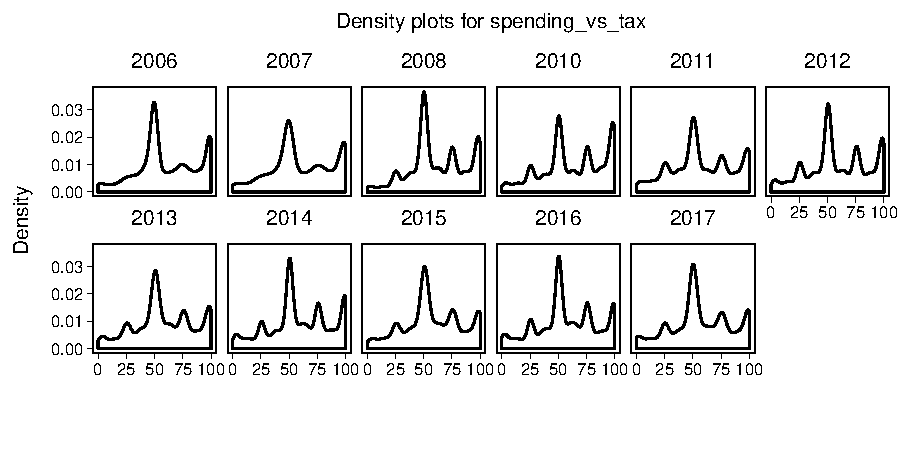
\includegraphics{guide_cumulative_cces_policy_preferences_files/figure-latex/unnamed-chunk-4-1} 

}

\caption{Density plots for question item}\label{fig:unnamed-chunk-4-1}
\end{figure}

Year-specific variable names and wording

\begin{longtable}[t]{rl>{\raggedright\arraybackslash}p{10cm}}
\caption{\label{tab:unnamed-chunk-4}spending\_vs\_tax: Year-specific wording}\\
\toprule
Year & Variable & Question wording\\
\midrule
\endfirsthead
\caption[]{spending\_vs\_tax: Year-specific wording \textit{(continued)}}\\
\toprule
Year & Variable & Question wording\\
\midrule
\endhead
\
\endfoot
\bottomrule
\endlastfoot
2006 & v4040 & If your state were to have a budget deficit this year it would have to raise taxes on income or sales or cut spending, such as on education, health care, welfare, and road construction. What would you prefer more raising taxes or cutting spending? Choose a point along the scale from 100 percent tax increases (and no spending cuts) to 100 percent spending cuts (and 0 percent no tax increases). The point in the middle means that any the budget should be balanced with equal amounts of spending cuts and tax increases.  If you are not sure, or don't know, please check here: [dk]\\
2007 & CC06\_V4040 & If your state were to have a budget deficit this year it would have to raise taxes on income or sales or cut spending, such as on education, health care, welfare, and road construction. What would you prefer more raising taxes or cutting spending? Choose a point along the scale from 100 percent tax increases (and no spending cuts) to 100 percent spending cuts (and 0 percent no tax increases). The point in the middle means that any the budget should be balanced with equal amounts of spending cuts and tax increases.\\
2008 & cc420 & If your state were to have a budget deficit this year it would have to raise taxes on income or sales or cut spending, such as on education, health care, welfare, and road construction. What would you prefer more, raising taxes or cutting spending? Choose a point along the scale from 100 percent tax increases (and no spending cuts) to 100 percent spending cuts (and no tax increases). The point in the middle means that the budget should be balanced with equal amounts of spending cuts and tax increases.  If you are not sure, or don't know, please check the box below... Values in range 0 to 100\\
2010 & CC415r & If your state were to have a budget deficit this year it would have to raise taxes on income or sales or cut spending, such as on education, health care, welfare, and road construction. What would you prefer more, raising taxes or cutting spending? Choose a point along the scale from 100 percent tax increases (and no spending cuts) to 100 percent spending cuts (and no tax increases). The point in the middle means that the budget should be balanced with equal amounts of spending cuts and tax increases. If you are not sure, or don't know, please check the box below Values in range 0 to 100\\
2011 & CC357 & Raise Taxes or Cut Spending Rule\\
2012 & CC415r & If your state were to have a budget deficit this year it would have to raise taxes on income and sales or cut spending, such as on education, health care, welfare, and road construction. What would you prefer more raising taxes or cutting spending? Choose a point along the scale from 100 percent tax increases (and no spending cuts) to 100 percent spending cuts (and no tax increases). The point in the middle means that the budget should be balanced with equal amounts of spending cuts and tax increases. If you are Not sure, or don't know, please check the 'not sure' box.\\
2013 & CC13\_323 & If your state were to have a budget deficit this year it would have to raise taxes on income and sales or cut spending, such as on education, health care, welfare, and road construction. What would you prefer more raising taxes or cutting spending? Choose a point along the scale from 100 percent tax increases (and no spending cuts) to 100 percent spending cuts (and no tax increases). The point in the middle means that the budget should be balanced with equal amounts of spending cuts and tax increases. If you are Not sure, or don't know, please check the 'not sure' box.\\
2014 & CC415r & If your state were to have a budget deficit this year it would have to raise taxes on income and sales or cut spending, such as on education, health care, welfare, and road construction. What would you prefer more raising taxes or cutting spending? Choose a point along the scale from 100 percent tax increases (and no spending cuts) to 100 percent spending cuts (and no tax increases). The point in the middle means that the budget should be balanced with equal amounts of spending cuts and tax increases. If you are Not sure, or don't know, please check the 'not sure' box.\\
2015 & CC15\_331 & If your state were to have a budget deficit this year it would have to raise taxes on income and sales or cut spending, such as on education, health care, welfare, and road construction. What would you prefer more raising taxes or cutting spending? Choose a point along the scale from 100 percent tax increases (and no spending cuts) to 100 percent spending cuts (and no tax increases). The point in the middle means that the budget should be balanced with equal amounts of spending cuts and tax increases. If you are Not sure, or don't know, please check the 'Not sure' box.\\
2016 & CC16\_415r & If your state were to have a budget deficit this year it would have to raise taxes on income and sales or cut spending, such as on education, health care, welfare, and road construction. What would you prefer more, raising taxes or cutting spending? Choose a point along the scale from 100\\
2017 & CC17\_343 & If your state were to have a budget deficit this year it would have to raise taxes on income and sales or cut spending, such as on education, health care, welfare, and road construction. What would you prefer more raising taxes or cutting spending? Choose a point along the scale from 100 percent tax increases (and no spending cuts) to 100 percent spending cuts (and no tax increases). The point in the middle means that the budget should be balanced with equal amounts of spending cuts and tax increases. If you are Not sure, or don't know, please check the 'Not sure' box.\\*
\end{longtable}

\subsubsection{spending\_cuts\_most}\label{spending_cuts_most}

Most preferred spending cut option (1=Defense, 2=Domestic, 3=Raise
taxes)

Years in data: 2006, 2007, 2008, 2010, 2011, 2012, 2013, 2014, 2015,
2017\begingroup\fontsize{10}{12}\selectfont

\begin{longtable}[t]{lcccccccccc}
\caption{\label{tab:unnamed-chunk-4}spending\_cuts\_most: Frequency table}\\
\toprule
Response & 2006 & 2007 & 2008 & 2010 & 2011 & 2012 & 2013 & 2014 & 2015 & 2017\\
\midrule
\endfirsthead
\caption[]{spending\_cuts\_most: Frequency table \textit{(continued)}}\\
\toprule
Response & 2006 & 2007 & 2008 & 2010 & 2011 & 2012 & 2013 & 2014 & 2015 & 2017\\
\midrule
\endhead
\
\endfoot
\bottomrule
\endlastfoot
Cut defense spending & 9,291 & 3,270 & 9,396 & 22,061 & 7,226 & 21,793 & 7,182 & 23,581 & 5,525 & 7,846\\
Cut domestic spending & 14,540 & 4,646 & 13,834 & 24,549 & 7,538 & 20,865 & 5,794 & 20,764 & 5,552 & 6,366\\
Raise taxes & 4,798 & 1,659 & 2,390 & 8,211 & 5,386 & 11,081 & 3,219 & 11,218 & 2,940 & 3,787\\
Borrow & 1,394 & 365 & 0 & 0 & 0 & 0 & 0 & 0 & 0 & 0\\*
\end{longtable}

\endgroup{}

Year-specific variable names and wording

\begin{longtable}[t]{rl>{\raggedright\arraybackslash}p{10cm}}
\caption{\label{tab:unnamed-chunk-4}spending\_cuts\_most: Year-specific wording}\\
\toprule
Year & Variable & Question wording\\
\midrule
\endfirsthead
\caption[]{spending\_cuts\_most: Year-specific wording \textit{(continued)}}\\
\toprule
Year & Variable & Question wording\\
\midrule
\endhead
\
\endfoot
\bottomrule
\endlastfoot
2006 & v4044 & What would you most prefer that Congress do - cut domestic spending, cut military spending, raise taxes, or borrow funds?\\
2007 & CC06\_V4044 & What would you most prefer that Congress do - cut domestic spending, cut military spending, raise taxes, or borrow funds?\\
2008 & cc309 & What would you most prefer that Congress do - cut domestic spending, cut military spending, or raise taxes?\\
2010 & CC328 & The federal budget is approximately 600 billion this year. If the Congress were to balance the budget it would have to consider cutting defense spending, cutting domestic spending (such as Medicare or Social Security), or raising taxes to cover the deficit. What would you most prefer that Congress do - cut domestic spending, cut defense spending, or raise taxes?\\
2011 & CC355a & Budget Balance 1\\
2012 & CC328 & The federal budget deficit is approximately 1 trillion this year. If the Congress were to balance the budget it would have to consider cutting defense spending, cutting domestic spending (such as Medicare and Social Security), or raising taxes to cover the deficit. What would you MOST prefer that Congress do - cut domestic spending, cut defense spending, or raise taxes\\
2013 & CC13\_331a & If your state were to have a budget deficit this year it would have to raise taxes on income and sales or cut spending, such as on education, health care, welfare, and road construction. What would you prefer more raising taxes or cutting spending? Choose a point along the scale from 100 percent tax increases (and no spending cuts) to 100 percent spending cuts (and no tax increases). The point in the middle means that the budget should be balanced with equal amounts of spending cuts and tax increases. If you are Not sure, or don't know, please check the 'not sure' box.\\
2014 & CC14\_329a & The federal budget deficit is approximately 500 billion this year. If the Congress were to balance the budget it would have to consider cutting defense spending, cutting domestic spending (such as Medicare and Social Security), or raising taxes to cover the deficit. What would you most prefer that Congress do - cut domestic spending, cut defense spending, or raise taxes?\\
2015 & CC15\_333a & The federal budget deficit is approximately 1 trillion this year. If the Congress were to balance the budget it would have to consider cutting defense spending, cutting domestic spending (such as Medicare and Social Security), or raising taxes to cover the deficit. What would you most prefer that Congress do - cut domestic spending, cut defense spending, or raise taxes?\\
2017 & CC17\_345a & The federal budget deficit is approximately 700 billion this year. If the Congress were to balance the budget it would have to consider cutting defense spending, cutting domestic spending (such as Medicare and Social Security), or raising taxes to cover the deficit. What would you most prefer that Congress do - cut domestic spending, cut defense spending, or raise taxes?\\*
\end{longtable}

\emph{Note: In 2006 and 2007, this question includes a fourth response
option, `Borrow'.}

\subsubsection{spending\_cuts\_least}\label{spending_cuts_least}

Least preferred spending cut option (1=Defense, 2=Domestic, 3=Raise
taxes)

Years in data: 2006, 2007, 2008, 2010, 2011, 2012, 2013, 2014, 2015,
2017\begingroup\fontsize{10}{12}\selectfont

\begin{longtable}[t]{lcccccccccc}
\caption{\label{tab:unnamed-chunk-4}spending\_cuts\_least: Frequency table}\\
\toprule
Response & 2006 & 2007 & 2008 & 2010 & 2011 & 2012 & 2013 & 2014 & 2015 & 2017\\
\midrule
\endfirsthead
\caption[]{spending\_cuts\_least: Frequency table \textit{(continued)}}\\
\toprule
Response & 2006 & 2007 & 2008 & 2010 & 2011 & 2012 & 2013 & 2014 & 2015 & 2017\\
\midrule
\endhead
\
\endfoot
\bottomrule
\endlastfoot
Cut defense spending & 6,870 & 2,051 & 4,808 & 8,062 & 4,721 & 10,493 & 2,665 & 11,694 & 3,232 & 4,035\\
Cut domestic spending & 3,245 & 1,208 & 5,933 & 17,016 & 7,446 & 19,130 & 6,131 & 18,583 & 4,939 & 6,943\\
Raise taxes & 7,924 & 2,629 & 14,919 & 29,550 & 7,800 & 23,876 & 7,343 & 25,098 & 5,917 & 7,010\\
Borrow & 11,041 & 3,821 & 0 & 0 & 0 & 0 & 0 & 0 & 0 & 0\\*
\end{longtable}

\endgroup{}

Year-specific variable names and wording

\begin{longtable}[t]{rl>{\raggedright\arraybackslash}p{10cm}}
\caption{\label{tab:unnamed-chunk-4}spending\_cuts\_least: Year-specific wording}\\
\toprule
Year & Variable & Question wording\\
\midrule
\endfirsthead
\caption[]{spending\_cuts\_least: Year-specific wording \textit{(continued)}}\\
\toprule
Year & Variable & Question wording\\
\midrule
\endhead
\
\endfoot
\bottomrule
\endlastfoot
2006 & v4046 & What do you least want Congress to do?\\
2007 & CC06\_V4046 & Should Congress cut spending, raise taxes, or borrow... What do you least want Congress to do?\\
2008 & cc310a & What do you least want Congress to do?\\
2010 & CC329 & The federal budget is approximately 600 billion this year. If the Congress were to balance the budget it would have to consider cutting defense spending, cutting domestic spending (such as Medicare or Social Security), or raising taxes to cover the deficit. What do you least want Congress to do?\\
2011 & CC355b & Budget Balance 2\\
2012 & CC329 & The federal budget deficit is approximately 1 trillion this year. If the Congress were to balance the budget it would have to consider cutting defense spending, cutting domestic spending (such as Medicare and Social Security), or raising taxes to cover the deficit. What would you LEAST prefer that Congress do - cut domestic spending, cut defense spending, or raise taxes\\
2013 & CC13\_331b & If the state had to raise taxes, what share of the tax increase should come from increased income taxes and what share from increased sales taxes? Choose a point along the scale from 100 percent from sales (and none from income) to 100 percent from income (and none from sales). The point in the middle means that any increase in taxes should come equally from sales and income taxes. If you are Not sure, or don't know, please check the 'not sure' box.\\
2014 & CC14\_329b & The federal budget deficit is approximately 500 billion this year. If the Congress were to balance the budget it would have to consider cutting defense spending, cutting domestic spending (such as Medicare and Social Security), or raising taxes to cover the deficit. What do you least want Congress to do?\\
2015 & CC15\_333b & The federal budget deficit is approximately 1 trillion this year. If the Congress were to balance the budget it would have to consider cutting defense spending, cutting domestic spending (such as Medicare and Social Security), or raising taxes to cover the deficit. What do you least want Congress to do?\\
2017 & CC17\_345b & The federal budget deficit is approximately 700 billion this year. If the Congress were to balance the budget it would have to consider cutting defense spending, cutting domestic spending (such as Medicare and Social Security), or raising taxes to cover the deficit. What do you least want Congress to do?\\*
\end{longtable}

\emph{Note: In 2006 and 2007, this question includes a fourth response
option, `Borrow'.}

\subsubsection{spending\_welfare}\label{spending_welfare}

Spending preferences on welfare (1 = Increase, 3 = Maintain, 5 =
Decrease)

Years in data: 2016, 2018\begingroup\fontsize{10}{12}\selectfont

\begin{longtable}[t]{lcc}
\caption{\label{tab:unnamed-chunk-4}spending\_welfare: Frequency table}\\
\toprule
Response & 2016 & 2018\\
\midrule
\endfirsthead
\caption[]{spending\_welfare: Frequency table \textit{(continued)}}\\
\toprule
Response & 2016 & 2018\\
\midrule
\endhead
\
\endfoot
\bottomrule
\endlastfoot
Greatly increase & 4,995 & 6,419\\
Slightly increase & 7,657 & 9,989\\
Maintain & 19,534 & 18,863\\
Slightly decrease & 10,176 & 8,393\\
Greatly decrease & 10,398 & 8,025\\*
\end{longtable}

\endgroup{}

Year-specific variable names and wording

\begin{longtable}[t]{rl>{\raggedright\arraybackslash}p{10cm}}
\caption{\label{tab:unnamed-chunk-4}spending\_welfare: Year-specific wording}\\
\toprule
Year & Variable & Question wording\\
\midrule
\endfirsthead
\caption[]{spending\_welfare: Year-specific wording \textit{(continued)}}\\
\toprule
Year & Variable & Question wording\\
\midrule
\endhead
\
\endfoot
\bottomrule
\endlastfoot
2016 & CC16\_426\_1 & State legislatures must make choices when making spending decisions on important state programs. Would you like your legislature to increase or decrease spending on the five areas below? Welfare\\
2018 & CC18\_426\_1 & State legislatures must make choices when making spending decisions on important state programs. Would you like your legislature to increase or decrease spending on the five areas below? Welfare\\*
\end{longtable}

\subsubsection{spending\_healthcare}\label{spending_healthcare}

Spending preferences on health care (1 = Increase, 3 = Maintain, 5 =
Decrease)

Years in data: 2016, 2018\begingroup\fontsize{10}{12}\selectfont

\begin{longtable}[t]{lcc}
\caption{\label{tab:unnamed-chunk-4}spending\_healthcare: Frequency table}\\
\toprule
Response & 2016 & 2018\\
\midrule
\endfirsthead
\caption[]{spending\_healthcare: Frequency table \textit{(continued)}}\\
\toprule
Response & 2016 & 2018\\
\midrule
\endhead
\
\endfoot
\bottomrule
\endlastfoot
Greatly increase & 13,550 & 19,862\\
Slightly increase & 14,765 & 14,109\\
Maintain & 16,781 & 12,689\\
Slightly decrease & 4,562 & 2,852\\
Greatly decrease & 3,096 & 2,158\\*
\end{longtable}

\endgroup{}

Year-specific variable names and wording

\begin{longtable}[t]{rl>{\raggedright\arraybackslash}p{10cm}}
\caption{\label{tab:unnamed-chunk-4}spending\_healthcare: Year-specific wording}\\
\toprule
Year & Variable & Question wording\\
\midrule
\endfirsthead
\caption[]{spending\_healthcare: Year-specific wording \textit{(continued)}}\\
\toprule
Year & Variable & Question wording\\
\midrule
\endhead
\
\endfoot
\bottomrule
\endlastfoot
2016 & CC16\_426\_2 & State legislatures must make choices when making spending decisions on important state programs. Would you like your legislature to increase or decrease spending on the five areas below? Health Care\\
2018 & CC18\_426\_2 & State legislatures must make choices when making spending decisions on important state programs. Would you like your legislature to increase or decrease spending on the five areas below? Health Care\\*
\end{longtable}

\subsubsection{spending\_education}\label{spending_education}

Spending preferences on education (1 = Increase, 3 = Maintain, 5 =
Decrease)

Years in data: 2016, 2018\begingroup\fontsize{10}{12}\selectfont

\begin{longtable}[t]{lcc}
\caption{\label{tab:unnamed-chunk-4}spending\_education: Frequency table}\\
\toprule
Response & 2016 & 2018\\
\midrule
\endfirsthead
\caption[]{spending\_education: Frequency table \textit{(continued)}}\\
\toprule
Response & 2016 & 2018\\
\midrule
\endhead
\
\endfoot
\bottomrule
\endlastfoot
Greatly increase & 18,166 & 21,875\\
Slightly increase & 15,144 & 14,467\\
Maintain & 14,460 & 11,805\\
Slightly decrease & 2,993 & 2,000\\
Greatly decrease & 1,969 & 1,500\\*
\end{longtable}

\endgroup{}

Year-specific variable names and wording

\begin{longtable}[t]{rl>{\raggedright\arraybackslash}p{10cm}}
\caption{\label{tab:unnamed-chunk-4}spending\_education: Year-specific wording}\\
\toprule
Year & Variable & Question wording\\
\midrule
\endfirsthead
\caption[]{spending\_education: Year-specific wording \textit{(continued)}}\\
\toprule
Year & Variable & Question wording\\
\midrule
\endhead
\
\endfoot
\bottomrule
\endlastfoot
2016 & CC16\_426\_3 & State legislatures must make choices when making spending decisions on important state programs. Would you like your legislature to increase or decrease spending on the five areas below? Education\\
2018 & CC18\_426\_3 & State legislatures must make choices when making spending decisions on important state programs. Would you like your legislature to increase or decrease spending on the five areas below? Education\\*
\end{longtable}

\subsubsection{spending\_police}\label{spending_police}

Spending preferences on law enforcement (1 = Increase, 3 = Maintain, 5 =
Decrease)

Years in data: 2016, 2018\begingroup\fontsize{10}{12}\selectfont

\begin{longtable}[t]{lcc}
\caption{\label{tab:unnamed-chunk-4}spending\_police: Frequency table}\\
\toprule
Response & 2016 & 2018\\
\midrule
\endfirsthead
\caption[]{spending\_police: Frequency table \textit{(continued)}}\\
\toprule
Response & 2016 & 2018\\
\midrule
\endhead
\
\endfoot
\bottomrule
\endlastfoot
Greatly increase & 11,346 & 11,764\\
Slightly increase & 17,417 & 17,309\\
Maintain & 19,428 & 18,443\\
Slightly decrease & 3,052 & 2,699\\
Greatly decrease & 1,449 & 1,405\\*
\end{longtable}

\endgroup{}

Year-specific variable names and wording

\begin{longtable}[t]{rl>{\raggedright\arraybackslash}p{10cm}}
\caption{\label{tab:unnamed-chunk-4}spending\_police: Year-specific wording}\\
\toprule
Year & Variable & Question wording\\
\midrule
\endfirsthead
\caption[]{spending\_police: Year-specific wording \textit{(continued)}}\\
\toprule
Year & Variable & Question wording\\
\midrule
\endhead
\
\endfoot
\bottomrule
\endlastfoot
2016 & CC16\_426\_4 & State legislatures must make choices when making spending decisions on important state programs. Would you like your legislature to increase or decrease spending on the five areas below? Law Enforcement\\
2018 & CC18\_426\_4 & State legislatures must make choices when making spending decisions on important state programs. Would you like your legislature to increase or decrease spending on the five areas below? Law Enforcement\\*
\end{longtable}

\subsubsection{spending\_infrastructure}\label{spending_infrastructure}

Spending preferences on transportation/infrastructure (1 = Increase, 3 =
Maintain, 5 = Decrease)

Years in data: 2016, 2018\begingroup\fontsize{10}{12}\selectfont

\begin{longtable}[t]{lcc}
\caption{\label{tab:unnamed-chunk-4}spending\_infrastructure: Frequency table}\\
\toprule
Response & 2016 & 2018\\
\midrule
\endfirsthead
\caption[]{spending\_infrastructure: Frequency table \textit{(continued)}}\\
\toprule
Response & 2016 & 2018\\
\midrule
\endhead
\
\endfoot
\bottomrule
\endlastfoot
Greatly increase & 13,764 & 16,899\\
Slightly increase & 17,798 & 19,015\\
Maintain & 17,793 & 13,851\\
Slightly decrease & 2,451 & 1,289\\
Greatly decrease & 921 & 582\\*
\end{longtable}

\endgroup{}

Year-specific variable names and wording

\begin{longtable}[t]{rl>{\raggedright\arraybackslash}p{10cm}}
\caption{\label{tab:unnamed-chunk-4}spending\_infrastructure: Year-specific wording}\\
\toprule
Year & Variable & Question wording\\
\midrule
\endfirsthead
\caption[]{spending\_infrastructure: Year-specific wording \textit{(continued)}}\\
\toprule
Year & Variable & Question wording\\
\midrule
\endhead
\
\endfoot
\bottomrule
\endlastfoot
2016 & CC16\_426\_5 & State legislatures must make choices when making spending decisions on important state programs. Would you like your legislature to increase or decrease spending on the five areas below? Transportation/Infrastructure\\
2018 & CC18\_426\_5 & State legislatures must make choices when making spending decisions on important state programs. Would you like your legislature to increase or decrease spending on the five areas below? Transportation/Infrastructure\\*
\end{longtable}\newpage

\subsection{Other}\label{other}

\subsubsection{affirmativeaction\_scale}\label{affirmativeaction_scale}

Opposition scale to affirmative action (1 = Strongly support, 7 =
Strongly oppose)

Years in data: 2006, 2007\begingroup\fontsize{10}{12}\selectfont

\begin{longtable}[t]{lcc}
\caption{\label{tab:unnamed-chunk-4}affirmativeaction\_scale: Frequency table}\\
\toprule
Response & 2006 & 2007\\
\midrule
\endfirsthead
\caption[]{affirmativeaction\_scale: Frequency table \textit{(continued)}}\\
\toprule
Response & 2006 & 2007\\
\midrule
\endhead
\
\endfoot
\bottomrule
\endlastfoot
Strongly support & 4,497 & 1,029\\
Support & 3,567 & 1,069\\
Somewhat support & 3,834 & 1,185\\
Neither support nor oppose & 6,623 & 1,726\\
Somewhat oppose & 3,145 & 839\\
Oppose & 3,903 & 1,125\\
Strongly oppose & 10,648 & 2,999\\*
\end{longtable}

\endgroup{}

Year-specific variable names and wording

\begin{longtable}[t]{rl>{\raggedright\arraybackslash}p{10cm}}
\caption{\label{tab:unnamed-chunk-4}affirmativeaction\_scale: Year-specific wording}\\
\toprule
Year & Variable & Question wording\\
\midrule
\endfirsthead
\caption[]{affirmativeaction\_scale: Year-specific wording \textit{(continued)}}\\
\toprule
Year & Variable & Question wording\\
\midrule
\endhead
\
\endfoot
\bottomrule
\endlastfoot
2006 & v3027 & Some people think that if a company has a history of discriminating against blacks when making hiring decisions, then they should be required to have an affirmative action program that gives blacks preference in hiring.    What do you think? Should companies that have discriminated against blacks have to have an affirmative action program?\\
2007 & CC06\_V3027 & Some people think that if a company has a history of discriminating against blacks when making hiring decisions, then they should be required to have an affirmative action program that gives blacks preference in hiring. What do you think? Should companies that have discriminated against blacks have to have an affirmative action program?\\*
\end{longtable}

\emph{Note: In 2006 and 2007, this question includes a fourth response
option, `Not sure', which has been re-coded as `NA' in this data set.}

\subsubsection{affirmativeaction}\label{affirmativeaction}

Opposition to affirmative action (1 = Support, 4 = Oppose)

Years in data: 2008, 2009, 2010, 2011, 2012, 2013,
2014\begingroup\fontsize{10}{12}\selectfont

\begin{longtable}[t]{lccccccc}
\caption{\label{tab:unnamed-chunk-4}affirmativeaction: Frequency table}\\
\toprule
Response & 2008 & 2009 & 2010 & 2011 & 2012 & 2013 & 2014\\
\midrule
\endfirsthead
\caption[]{affirmativeaction: Frequency table \textit{(continued)}}\\
\toprule
Response & 2008 & 2009 & 2010 & 2011 & 2012 & 2013 & 2014\\
\midrule
\endhead
\
\endfoot
\bottomrule
\endlastfoot
Strongly support & 2,997 & 1,581 & 6,638 & 2,251 & 7,448 & 1,993 & 8,116\\
Somewhat support & 6,985 & 3,236 & 12,985 & 4,887 & 13,797 & 4,176 & 14,161\\
Somewhat oppose & 6,235 & 3,392 & 13,326 & 5,406 & 14,183 & 4,219 & 14,135\\
Strongly oppose & 9,384 & 5,541 & 22,324 & 7,579 & 18,869 & 5,930 & 19,591\\*
\end{longtable}

\endgroup{}

Year-specific variable names and wording

\begin{longtable}[t]{rl>{\raggedright\arraybackslash}p{10cm}}
\caption{\label{tab:unnamed-chunk-4}affirmativeaction: Year-specific wording}\\
\toprule
Year & Variable & Question wording\\
\midrule
\endfirsthead
\caption[]{affirmativeaction: Year-specific wording \textit{(continued)}}\\
\toprule
Year & Variable & Question wording\\
\midrule
\endhead
\
\endfoot
\bottomrule
\endlastfoot
2008 & cc313 & Affirmative action programs give preference to racial minorities and to women in employment and college admissions in order to correct for discrimination. Do you support or oppose affirmative action?\\
2009 & cc09\_55 & Affirmative Action\\
2010 & CC327 & Affirmative action programs give preference to racial minorities in employment and college admissions in order to correct for past discrimination. Do you support or oppose affirmative action?\\
2011 & CC354 & Affirmative Action\\
2012 & CC327 & Affirmative action programs give preference to racial minorities in employment and college admissions in order to correct for past discrimination. Do you support or oppose affirmative action?\\
2013 & CC330 & Affirmative action programs give preference to racial minorities in employment and college admissions in order to correct for past discrimination. Do you support or oppose affirmative action?\\
2014 & CC14\_328 & Affirmative action programs give preference to racial minorities in employment and college admissions in order to correct for past discrimination. Do you support or oppose affirmative action?\\*
\end{longtable}

\subsubsection{gaymarriage\_scale}\label{gaymarriage_scale}

Opposition scale to gay marriage (1=Strongly support, 4=Strongly oppose)

Years in data: 2006, 2007\begingroup\fontsize{10}{12}\selectfont

\begin{longtable}[t]{lcc}
\caption{\label{tab:unnamed-chunk-4}gaymarriage\_scale: Frequency table}\\
\toprule
Response & 2006 & 2007\\
\midrule
\endfirsthead
\caption[]{gaymarriage\_scale: Frequency table \textit{(continued)}}\\
\toprule
Response & 2006 & 2007\\
\midrule
\endhead
\
\endfoot
\bottomrule
\endlastfoot
Strongly support & 5,841 & 1,958\\
Somewhat support & 1,567 & 529\\
Somewhat oppose & 1,457 & 506\\
Stongly oppose & 6,929 & 2,893\\
Don't know & 417 & 143\\*
\end{longtable}

\endgroup{}

Year-specific variable names and wording

\begin{longtable}[t]{rl>{\raggedright\arraybackslash}p{10cm}}
\caption{\label{tab:unnamed-chunk-4}gaymarriage\_scale: Year-specific wording}\\
\toprule
Year & Variable & Question wording\\
\midrule
\endfirsthead
\caption[]{gaymarriage\_scale: Year-specific wording \textit{(continued)}}\\
\toprule
Year & Variable & Question wording\\
\midrule
\endhead
\
\endfoot
\bottomrule
\endlastfoot
2006 & v2103 & President Bush recently spoke out in favor of a Constitutional Amendment defining marriage as strictly between a man and a woman. Do you support or oppose a Constitutional amendment banning gay marriage?\\
2007 & CC06\_V2103 & President Bush recently spoke out in favor of a Constitutional Amendment defining marriage as strictly between a man and a woman. Do you support or oppose a Constitutional amendment banning gay marriage?\\*
\end{longtable}

\subsubsection{gaymarriage}\label{gaymarriage}

Opposition to gay marriage

Years in data: 2008, 2009, 2010, 2011, 2012, 2013, 2014, 2015,
2016\begingroup\fontsize{10}{12}\selectfont

\begin{longtable}[t]{lccccccccc}
\caption{\label{tab:unnamed-chunk-4}gaymarriage: Frequency table}\\
\toprule
Response & 2008 & 2009 & 2010 & 2011 & 2012 & 2013 & 2014 & 2015 & 2016\\
\midrule
\endfirsthead
\caption[]{gaymarriage: Frequency table \textit{(continued)}}\\
\toprule
Response & 2008 & 2009 & 2010 & 2011 & 2012 & 2013 & 2014 & 2015 & 2016\\
\midrule
\endhead
\
\endfoot
\bottomrule
\endlastfoot
Support & 12,251 & 7,674 & 31,830 & 12,208 & 28,085 & 9,308 & 32,810 & 8,248 & 41,718\\
Oppose & 13,430 & 6,067 & 23,328 & 7,942 & 25,857 & 6,867 & 22,860 & 5,841 & 22,407\\*
\end{longtable}

\endgroup{}

Year-specific variable names and wording

\begin{longtable}[t]{rl>{\raggedright\arraybackslash}p{10cm}}
\caption{\label{tab:unnamed-chunk-4}gaymarriage: Year-specific wording}\\
\toprule
Year & Variable & Question wording\\
\midrule
\endfirsthead
\caption[]{gaymarriage: Year-specific wording \textit{(continued)}}\\
\toprule
Year & Variable & Question wording\\
\midrule
\endhead
\
\endfoot
\bottomrule
\endlastfoot
2008 & cc316f & Constitutional Amendment banning Gay Marriage\\
2009 & cc09\_54 & Gay Marriage\\
2010 & CC326 & Do you support a Constitutional Amendment banning Gay Marriage?\\
2011 & CC353 & Gay Marriage\\
2012 & CC326 & Do you favor or oppose allowing gays and lesbians to marry legally?\\
2013 & CC329 & Do you favor or oppose allowing gays and lesbians to marry legally?\\
2014 & CC14\_327 & Do you favor or oppose allowing gays and lesbians to marry legally?\\
2015 & CC15\_325 & Do you favor or oppose allowing gays and lesbians to marry legally?\\
2016 & CC16\_335 & Do you favor or oppose allowing gays and lesbians to marry legally?\\*
\end{longtable}

\emph{Note: In 2008, this question includes a third response option,
`Not sure', which has been re-coded as `NA' in this data set.
Additionally, from 2012 onward, question wording switches from asking
respondents about their support of banning gay marriage, to their
support of gay marriage.}

\subsubsection{incometax\_vs\_salestax}\label{incometax_vs_salestax}

Preference scale from 0 (increase income tax) to 100 (increase sales
tax)

Years in data: 2006, 2007, 2008, 2010, 2011, 2012, 2013, 2014, 2015,
2016, 2017

\begin{figure}

{\centering 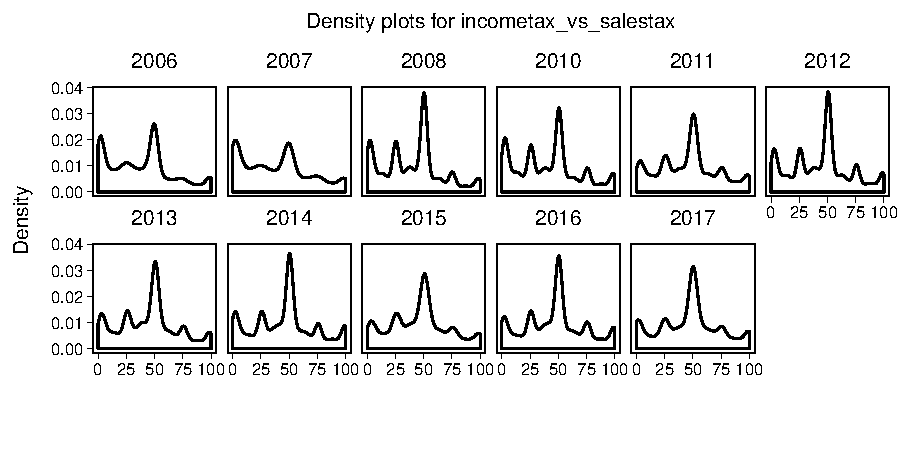
\includegraphics{guide_cumulative_cces_policy_preferences_files/figure-latex/unnamed-chunk-4-2} 

}

\caption{Density plots for question item}\label{fig:unnamed-chunk-4-2}
\end{figure}

Year-specific variable names and wording

\begin{longtable}[t]{rl>{\raggedright\arraybackslash}p{10cm}}
\caption{\label{tab:unnamed-chunk-4}incometax\_vs\_salestax: Year-specific wording}\\
\toprule
Year & Variable & Question wording\\
\midrule
\endfirsthead
\caption[]{incometax\_vs\_salestax: Year-specific wording \textit{(continued)}}\\
\toprule
Year & Variable & Question wording\\
\midrule
\endhead
\
\endfoot
\bottomrule
\endlastfoot
2006 & v4042 & If the state had to raise taxes, which taxes should it increase? Suppose that your state government has to raise some combination of sales taxes and individual income taxes in the coming year. What share of the tax increase should come from increased income taxes and what share from increased sales taxes? Choose a point along the scale from 100 percent from sales (and none from income) to 100 percent from income (and none from sales). The point in the middle means that any increase in taxes should come equally from sales and income taxes.  If you are not sure, or don't know, please check here: [dk]\\
2007 & CC06\_V4042 & If the state had to raise taxes, which taxes should it increase? Suppose that your state government has to raise some combination of sales taxes and individual income taxes in the coming year. What share of the tax increase should come from increased income taxes and what share from increased sales taxes? Choose a point along the scale from 100 percent from sales (and none from income) to 100 percent from income (and none from sales). The point in the middle means that any increase in taxes should come equally from sales and income taxes.\\
2008 & cc421 & If the state had to raise taxes, what share of the tax increase should come from increased income taxes and what share from increased sales taxes? Choose a point along the scale from 100 percent from sales (and none from income) to 100 percent from income (and none from sales). The point in the middle means that any increase in taxes should come equally from sales and income taxes.  If you are not sure, or don't know, please check the box below... Values in range 0 to 100\\
2010 & CC416r & If the state had to raise taxes, what share of the tax increase should come from increased income taxes and what share from increased sales taxes? Choose a point along the scale from 100 percent from sales (and none from income) to 100 percent from income (and none from sales). The point in the middle means that any increase in taxes should come equally from sales and income taxes. If you are not sure, or don't know, please check the box below Values in range 0 to 100\\
2011 & CC358 & Income vs Sales Tax Rule\\
2012 & CC416r & If the state had to raise taxes, what share of the tax increase should come from increased income taxes and what share from increased sales taxes? Choose a point along the scale from 100 percent from sales (and none from income) to 100 percent from income (and none from sales). The point in the middle means that any increase in taxes should come equally from sales and income taxes. If you are Not sure, or don't know, please check the 'not sure' box.\\
2013 & CC13\_324 & If the state had to raise taxes, what share of the tax increase should come from increased income taxes and what share from increased sales taxes? Choose a point along the scale from 100 percent from sales (and none from income) to 100 percent from income (and none from sales). The point in the middle means that any increase in taxes should come equally from sales and income taxes. If you are Not sure, or don't know, please check the 'not sure' box.\\
2014 & CC416r & If the state had to raise taxes, what share of the tax increase should come from increased income taxes and what share from increased sales taxes? Choose a point along the scale from 100 percent from sales (and none from income) to 100 percent from income (and none from sales). The point in the middle means that any increase in taxes should come equally from sales and income taxes. If you are Not sure, or don't know, please check the 'not sure' box.\\
2015 & CC15\_332 & If the state had to raise taxes, what share of the tax increase should come from increased income taxes and what share from increased sales taxes? Choose a point along the scale from 100 percent from sales (and none from income) to 100 percent from income (and none from sales). The point in the middle means that any increase in taxes should come equally from sales and income taxes. If you are Not sure, or don't know, please check the 'Not sure' box.\\
2016 & CC16\_416r & If the state had to raise taxes, what share of the tax increase should come from increased income taxes and what share from increased sales taxes? Choose a point along the scale from 100\\
2017 & CC17\_344 & If the state had to raise taxes, what share of the tax increase should come from increased income taxes and what share from increased sales taxes? Choose a point along the scale from 100 percent from sales (and none from income) to 100 percent from income (and none from sales). The point in the middle means that any increase in taxes should come equally from sales and income taxes. If you are Not sure, or don't know, please check the 'Not sure' box.\\*
\end{longtable}

\subsubsection{repealaca}\label{repealaca}

Repeal the Affordable Care Act

Years in data: 2012, 2013, 2014, 2015, 2016, 2017, 2018,
2019\begingroup\fontsize{10}{12}\selectfont

\begin{longtable}[t]{lcccccccc}
\caption{\label{tab:unnamed-chunk-4}repealaca: Frequency table}\\
\toprule
Response & 2012 & 2013 & 2014 & 2015 & 2016 & 2017 & 2018 & 2019\\
\midrule
\endfirsthead
\caption[]{repealaca: Frequency table \textit{(continued)}}\\
\toprule
Response & 2012 & 2013 & 2014 & 2015 & 2016 & 2017 & 2018 & 2019\\
\midrule
\endhead
\
\endfoot
\bottomrule
\endlastfoot
Support & 23,288 & 8,506 & 28,950 & 7,881 & 34,693 & 8,026 & 24,887 & 8,349\\
Oppose & 28,884 & 7,321 & 26,879 & 6,166 & 29,816 & 10,020 & 35,039 & 9,501\\*
\end{longtable}

\endgroup{}

Year-specific variable names and wording

\begin{longtable}[t]{rl>{\raggedright\arraybackslash}p{10cm}}
\caption{\label{tab:unnamed-chunk-4}repealaca: Year-specific wording}\\
\toprule
Year & Variable & Question wording\\
\midrule
\endfirsthead
\caption[]{repealaca: Year-specific wording \textit{(continued)}}\\
\toprule
Year & Variable & Question wording\\
\midrule
\endhead
\
\endfoot
\bottomrule
\endlastfoot
2012 & CC332G & Congress Considered many important bills over the past two years. For each of the following tell us whether you support or oppose the legislation in principle. Repeal Affordable Care Act. Would repeal the Affordable Care Act.\\
2013 & CC332C & Congress considered many important bills over the past few years. For each of the following tell us whether you support or oppose the legislation in principle. Repeal Affordable Care Act. Would repeal the Affordable Care Act.\\
2014 & CC14\_324\_1 & The Affordable Health Care Act was passed into law in 2010. It does the following: Requires Americans to obtain health insurance. Prevents insurance companies from denying coverage for pre-existing conditions. Allows people to keep current health insurance and care provider. Sets up national health insurance option for those without coverage, but allows states the option to implement their own insurance system.\\
2015 & CC15\_327A & Congress considered many important bills over the past few years. For each of the following tell us whether you support or oppose the legislation in principle. Repeal Affordable Care Act. Would repeal the Affordable Care Act.\\
2016 & CC16\_351I & Congress considers many issues. If you were in Congress would you vote FOR or AGAINST each of the following? Repeal Affordable Care Act. Would repeal the Affordable Care Act of 2009 (also known as Obamacare).\\
2017 & CC17\_340A & Congress considered many important bills over the past few years. For each of the following tell us whether you support or oppose the legislation in principle. Repeal Affordable Care Act. Would repeal the Affordable Care Act.\\
2018 & CC18\_327c & Thinking now about health care policy, would you support or oppose each of the following proposals? Health Care – Repeal the entire Affordable Care Act.\\
2019 & CC19\_327d & Repeal the entire Affordable Care Act.\\*
\end{longtable}

\emph{Note: In 2014 alone, question wording switches from asking
respondents about their support for repealing the Affordable Care Act,
to their support for the Act.}

\end{document}
